\documentclass[12pt]{article}
\usepackage{hyperref}
\usepackage[warn]{mathtext}
\usepackage[T2A]{fontenc}
\usepackage[utf8]{inputenc}
\usepackage[russian]{babel}
\usepackage{cite}
\usepackage{amsfonts}
\usepackage{lineno}
\usepackage{subfig}
\usepackage{graphicx}
\usepackage{xcolor}
\usepackage{bm}
\usepackage{graphicx}
\usepackage{amssymb}
\usepackage{hyperref}
\usepackage[left=2cm,right=2cm,top=2cm,bottom=2cm]{geometry}
\usepackage{indentfirst}
\DeclareSymbolFont{T2Aletters}{T2A}{cmr}{m}{it}

\DeclareGraphicsExtensions{.png,.jpg,.svg,.pdf}
\graphicspath{{spectres/}}
\author{Карцев Вадим}
\title{Лабораторная работа 1.2

Исследование эффекта Комптона}

\begin{document}

  \maketitle

  \tableofcontents

  \vspace{1cm}

  \textbf{Цель работы:} исследовать энергетический спектр $\gamma$-квантов,
  рассеянных на графите, определение зависимости энергии $\gamma$-квантов в
  зависимости от угла рассеяния и энергии покоя частиц, на которых происходит
  комптоновское рассеяние.

  \textbf{В работе используется:} контейнер с $^{137}Cs$, сцинтилляционный
  спектрометр, компъютер, ФЭУ, рассеивающая мишень.

  \section{Аннотация}

    В ходе работы с помощью сцинтилляционного спектрометра были изучены спектры
    рассеянных на графите $\gamma$-квантов. С их помощью была получена
    согласованная с теорией зависимость энергии от угла рассеяния и значение
    энергии покоя графита $mc^2 = (488,51 \pm 13,43) кэВ$

  \section{Теоретическая справка}

    \textbf{Эффект Комптона} -- явление увеличения длины волны рассеянного
    излучения по сравнению с падающим. Он интерпретируется как результат
    упругого соударения двух частиц -- $\gamma$-кванта и свободного электрона.

    Пусть электрон до соударения покоился, а $\gamma$-квант имел начальную
    энергию $\hbar \omega_0$ и импульс $\hbar \omega_0 / c$. После соударения
    электрон приобретает энергию $\gamma m c^2$, где $\gamma =
    (1 \beta^2)^{1/2}$, $\beta = v / c$, а $\gamma$-квант рассеивается на
    некторый угол $\theta$ по отношению к первоначальному направлению движения.
    Энергия и импульс рассеянного излучения -- $\propto \omega_1$. Запишем для
    рассматриваемого процесса законы сохранения энергии и импульса:

    $$
      mc^2 + \hbar \omega_0 = \gamma m c^2 + \hbar \omega_1
    $$

    $$
      \frac{\hbar \omega_0}{c} = \gamma m v \cos \varphi +
      \frac{\hbar \omega_1}{c} \cos \theta
    $$

    $$
      \gamma m v \sin \varphi = \frac{\hbar \omega_1}{c} \sin \theta
    $$

    Решая эти уравнения и переходя от частот к длинам волн, получим изменение
    длины рассеянного излучения

    \begin{equation}
      \Delta \lambda = \lambda_1 - \lambda_0 = \frac{h}{mc} (1 - \cos \theta) =
      \Lambda (1 - \cos \theta)
      \label{th:eq1}
    \end{equation}

    где $\Lambda_k = \frac{h}{mc} = 2.4210^{-10} см$ -- комптоновская длина
    волны электрона.

    Основной целью работы является проверка соотношения \ref{th:eq1}.
    Преобразуем его от длин волн к энергии $\gamma$-квантов.

    \begin{equation}
      \frac{1}{\varepsilon(\theta)} - \frac{1}{\varepsilon_0} = 1 - \cos \theta
      \label{th:eq2}
    \end{equation}

    где $\varepsilon_0 = E_0 / (mc^2)$ -- энергия $\gamma$-квантов, падающих на
    рассеиватель (в единицах $mc^2$), $\varepsilon(\theta)$ -- выраженная в тех
    же единицах энергия квантов, испытавших комптоновское рассеяние на угол
    $\theta$, $m$ -- масса электрона.

  \section{Экспериметальная установка}

    В лабораторной работе источником излучения служит $^{137}Cs$, испускающий
    поток $\gamma$-квантов с энергией $661,6 кэВ$. Пучок после выхода из
    коллиматорного отверстия попадает на графитовую мишень и рассеивается.
    Кванты, испытавшие комптоновское рассеяние, регистрируются сцинтилляционным
    счетчиком и приходят на ФЭУ. Сигналы, возникающие в ФЭУ, передаются на ПК
    для последующего спектрального анализа.

    \begin{figure}[h!]
      \begin{minipage}[t]{0.49\linewidth}
        \center{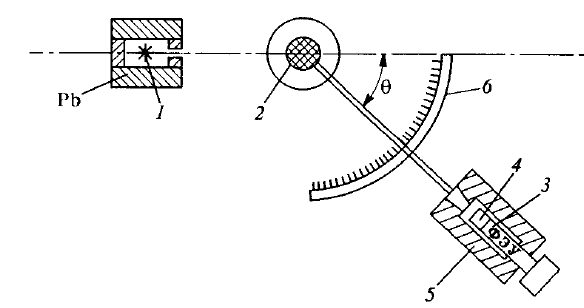
\includegraphics[width = \linewidth]{scheme.png}}\\
        Рис 1. Принципиальная схема установки
        \label{fig:scheme}
      \end{minipage}
      \begin{minipage}[t]{0.49\linewidth}
        \center{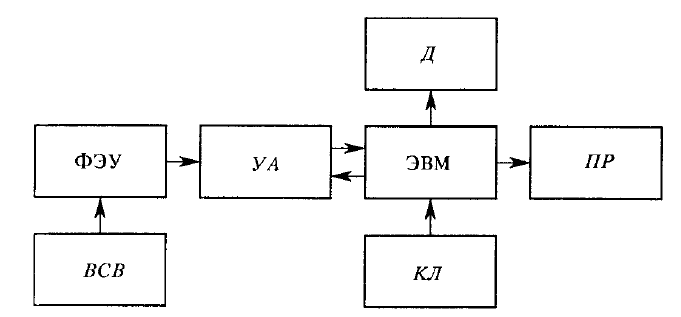
\includegraphics[width = \linewidth]{block_scheme.png}}\\
        Рис 2. Блок-схема установки
        \label{fig:block_scheme}
      \end{minipage}
    \end{figure}

    Сцинтилляционный счетчик установлен на подвижном рычаге, с помощью которого
    мы можем установить счетчик под необходимым углом к направлению потока
    $\gamma$-излучения.

  \section{Ход работы и обработка результатов}

    С помощью сцинтилляционного счетчика проведем замеры спектра и выясним
    зависимость положения фотопика от угла, под которым мы исследуем спектр
    рассеянных $\gamma$-лучей.

    Длительность замера спектра для каждого угла выберем такой, чтобы фотопик
    был в полной мере различим на спектрограмме.

    По спектрограммам на стр. \pageref{add:spectres} определим расположения
    фотопиков для раличных углов рассеяния.
    Ниже приведена таблица с результатами измерений для всех углов $\theta$.
    Погрешность измерения угла будем считать как половину деления разметки
    измерительного стола $\sigma_{\theta} = 0,5^{\circ}$.
    Погрешность положения фотопика возьмем как половину ширины вершины фотопика.
    Значения погрешности положения также приведены в таблице ниже.\\

    \begin{tabular}{|c||c|c|c|c|c|c|c|c|c|c|c|c|c|}
      \hline
      $\theta$ & $0^{\circ}$ & $10^{\circ}$ & $20^{\circ}$ & $30^{\circ}$ &
      $40^{\circ}$ & $50^{\circ}$ & $60^{\circ}$ & $70^{\circ}$ & $80^{\circ}$ &
      $90^{\circ}$ & $100^{\circ}$ & $110^{\circ}$ & $120^{\circ}$ \\ \hline
      $N$ & $912$ & $868$ & $790$ & $751$ & $665$ & $594$ & $536$ & $463$ &
      $424$ & $385$ & $353$ & $319$ & $282$ \\ \hline
      $\sigma_N$ & $8$ & $7$ & $20$ & $6$ & $8$ & $5$ & $4$ & $6$ & $6$ & $3$ &
      $5$ & $2$ & $6$ \\
      \hline
    \end{tabular}\\

    Погрешность для $1/N$ и $1 - \cos\theta$ будут считаться по формулам

    $$
      \sigma_{1/N} = \frac{1}{N} \varepsilon_N = \frac{1}{N} \frac{\sigma_N}{N}
      = \frac{\sigma_N}{N^2}; \hspace{0.5cm}
      \sigma_{1 - \cos\theta} = \sin(\theta) \sigma_{\theta}.
    $$

    \begin{figure}[h!]
      \center{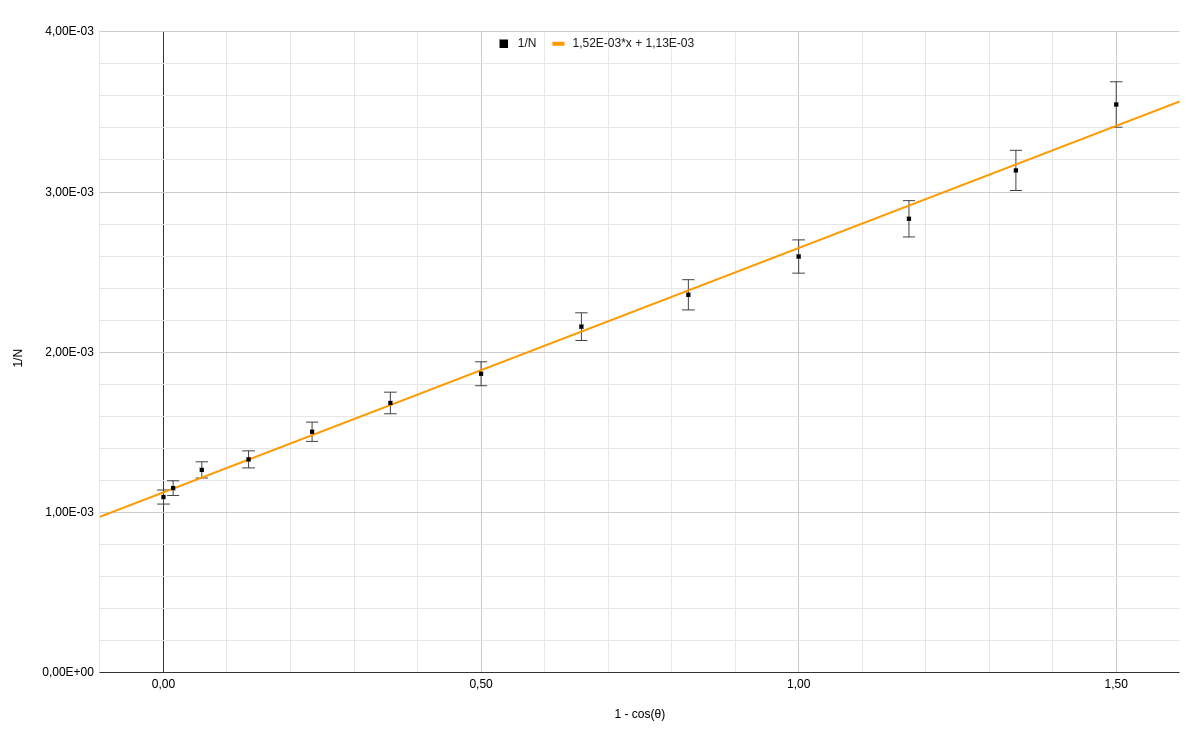
\includegraphics[width = \linewidth]{plot.png}}\\
      Рис 3. Зависимость $\frac{1}{N} \left(1 - \cos \theta \right)$
      \label{fig:plot}
    \end{figure}

    По МНК получим коэффициент наклона и точку пересечения прямой с осью Y.
    Также вычислим погрешности для этих значений.

    $$
      A = \frac{\left<xy\right> - \left<x\right>\left<y\right>}{\left<x^2\right>
      - \left<x\right>^2}; \hspace{0.5cm} \sigma_A = \frac{1}{\sqrt{n}}
      \sqrt{\frac{\left<y^2\right> - \left<y\right>^2}{\left<x^2\right> -
      \left<x\right>^2} - A^2}
    $$

    $$
      \frac{1}{N(0)} = \left<y\right> - A \left<x\right>; \hspace{0.5cm}
      \sigma_{1/N(0)} = \sigma_A \sqrt{\left<x^2\right>}
    $$

    Здесь для удобства мы произвели переименование $x \stackrel{def}{\equiv}
    1 - \cos \theta$, $y \stackrel{def}{\equiv} 1 / N$.

    Из этих формул рассчитаем значения угла наклона и пересечения прямой с осью
    Y с погрешностями.

    $$
      A = (152,5 \pm 2,8) \cdot 10^{-5}; \hspace{0.5cm}
      \frac{1}{N(0)} = (112,6 \pm 2,2) \cdot 10^{-5}
    $$

    С помощью полученных значений для прямой аппроксимации вычислим наилучшие
    значения для положения фотопика при углах $0^{\circ}$ и $90^{\circ}$.

    $$
      N(0^{\circ}) = 888,28 \pm 17,57; \hspace{0.5cm}
      N(90^{\circ}) = 377,30 \pm 7,21
    $$

    Из вычисленных значений для $N(0^{\circ})$ и $N(90^{\circ})$ получим
    значение $mc^2$ и погрешность для него по следующим формулам

    $$
      mc^2 = E_{\gamma} \frac{N(90^{\circ})}{N(0^{\circ}) - N(90^{\circ})};
      \hspace{0.5cm}
      \sigma_{mc^2} = mc^2 \sqrt{\varepsilon_{N(0^{\circ})}^2 +
      \varepsilon_{N(90^{\circ})}^2}
    $$

    где

    $$
      \varepsilon_{N(0^{\circ})} = \frac{\sigma_{N(0^{\circ})}}{N(0^{\circ})};
      \hspace{0.5cm}
      \varepsilon_{N(90^{\circ})} = \frac{\sigma_{N(90^{\circ})}}{N(90^{\circ})}
    $$

    Таким образом получим результат $mc^2 = (488,51 \pm 13,43) кэВ$. Полученный
    результат имеет относительную погрешность $\varepsilon_{mc^2} = 2,75\%$.

  \section{Вывод}

    В ходе выполнения работы было исследовано явление комптоновского рассеяния
    $\gamma$-квантов на графитовой мишени, подтверждена теоретическая
    зависимость распределения энергии $\gamma$-квантов по углам рассеяния, а
    также вычислена энергия покоя электрона $mc^2 = (488,51 \pm 13,43) кэВ$.
    Теоретическое значение энергии покоя электрона $mc^2_{теор} = 511 кэВ$, что
    в рамках двойной погрешности согласуется с полученным экспериментальным
    путем значением.

  \newpage
  \section{Приложение}
  \label{add:spectres}

  \begin{figure}[h!]
    \begin{minipage}[h]{0.32\linewidth}
      \center{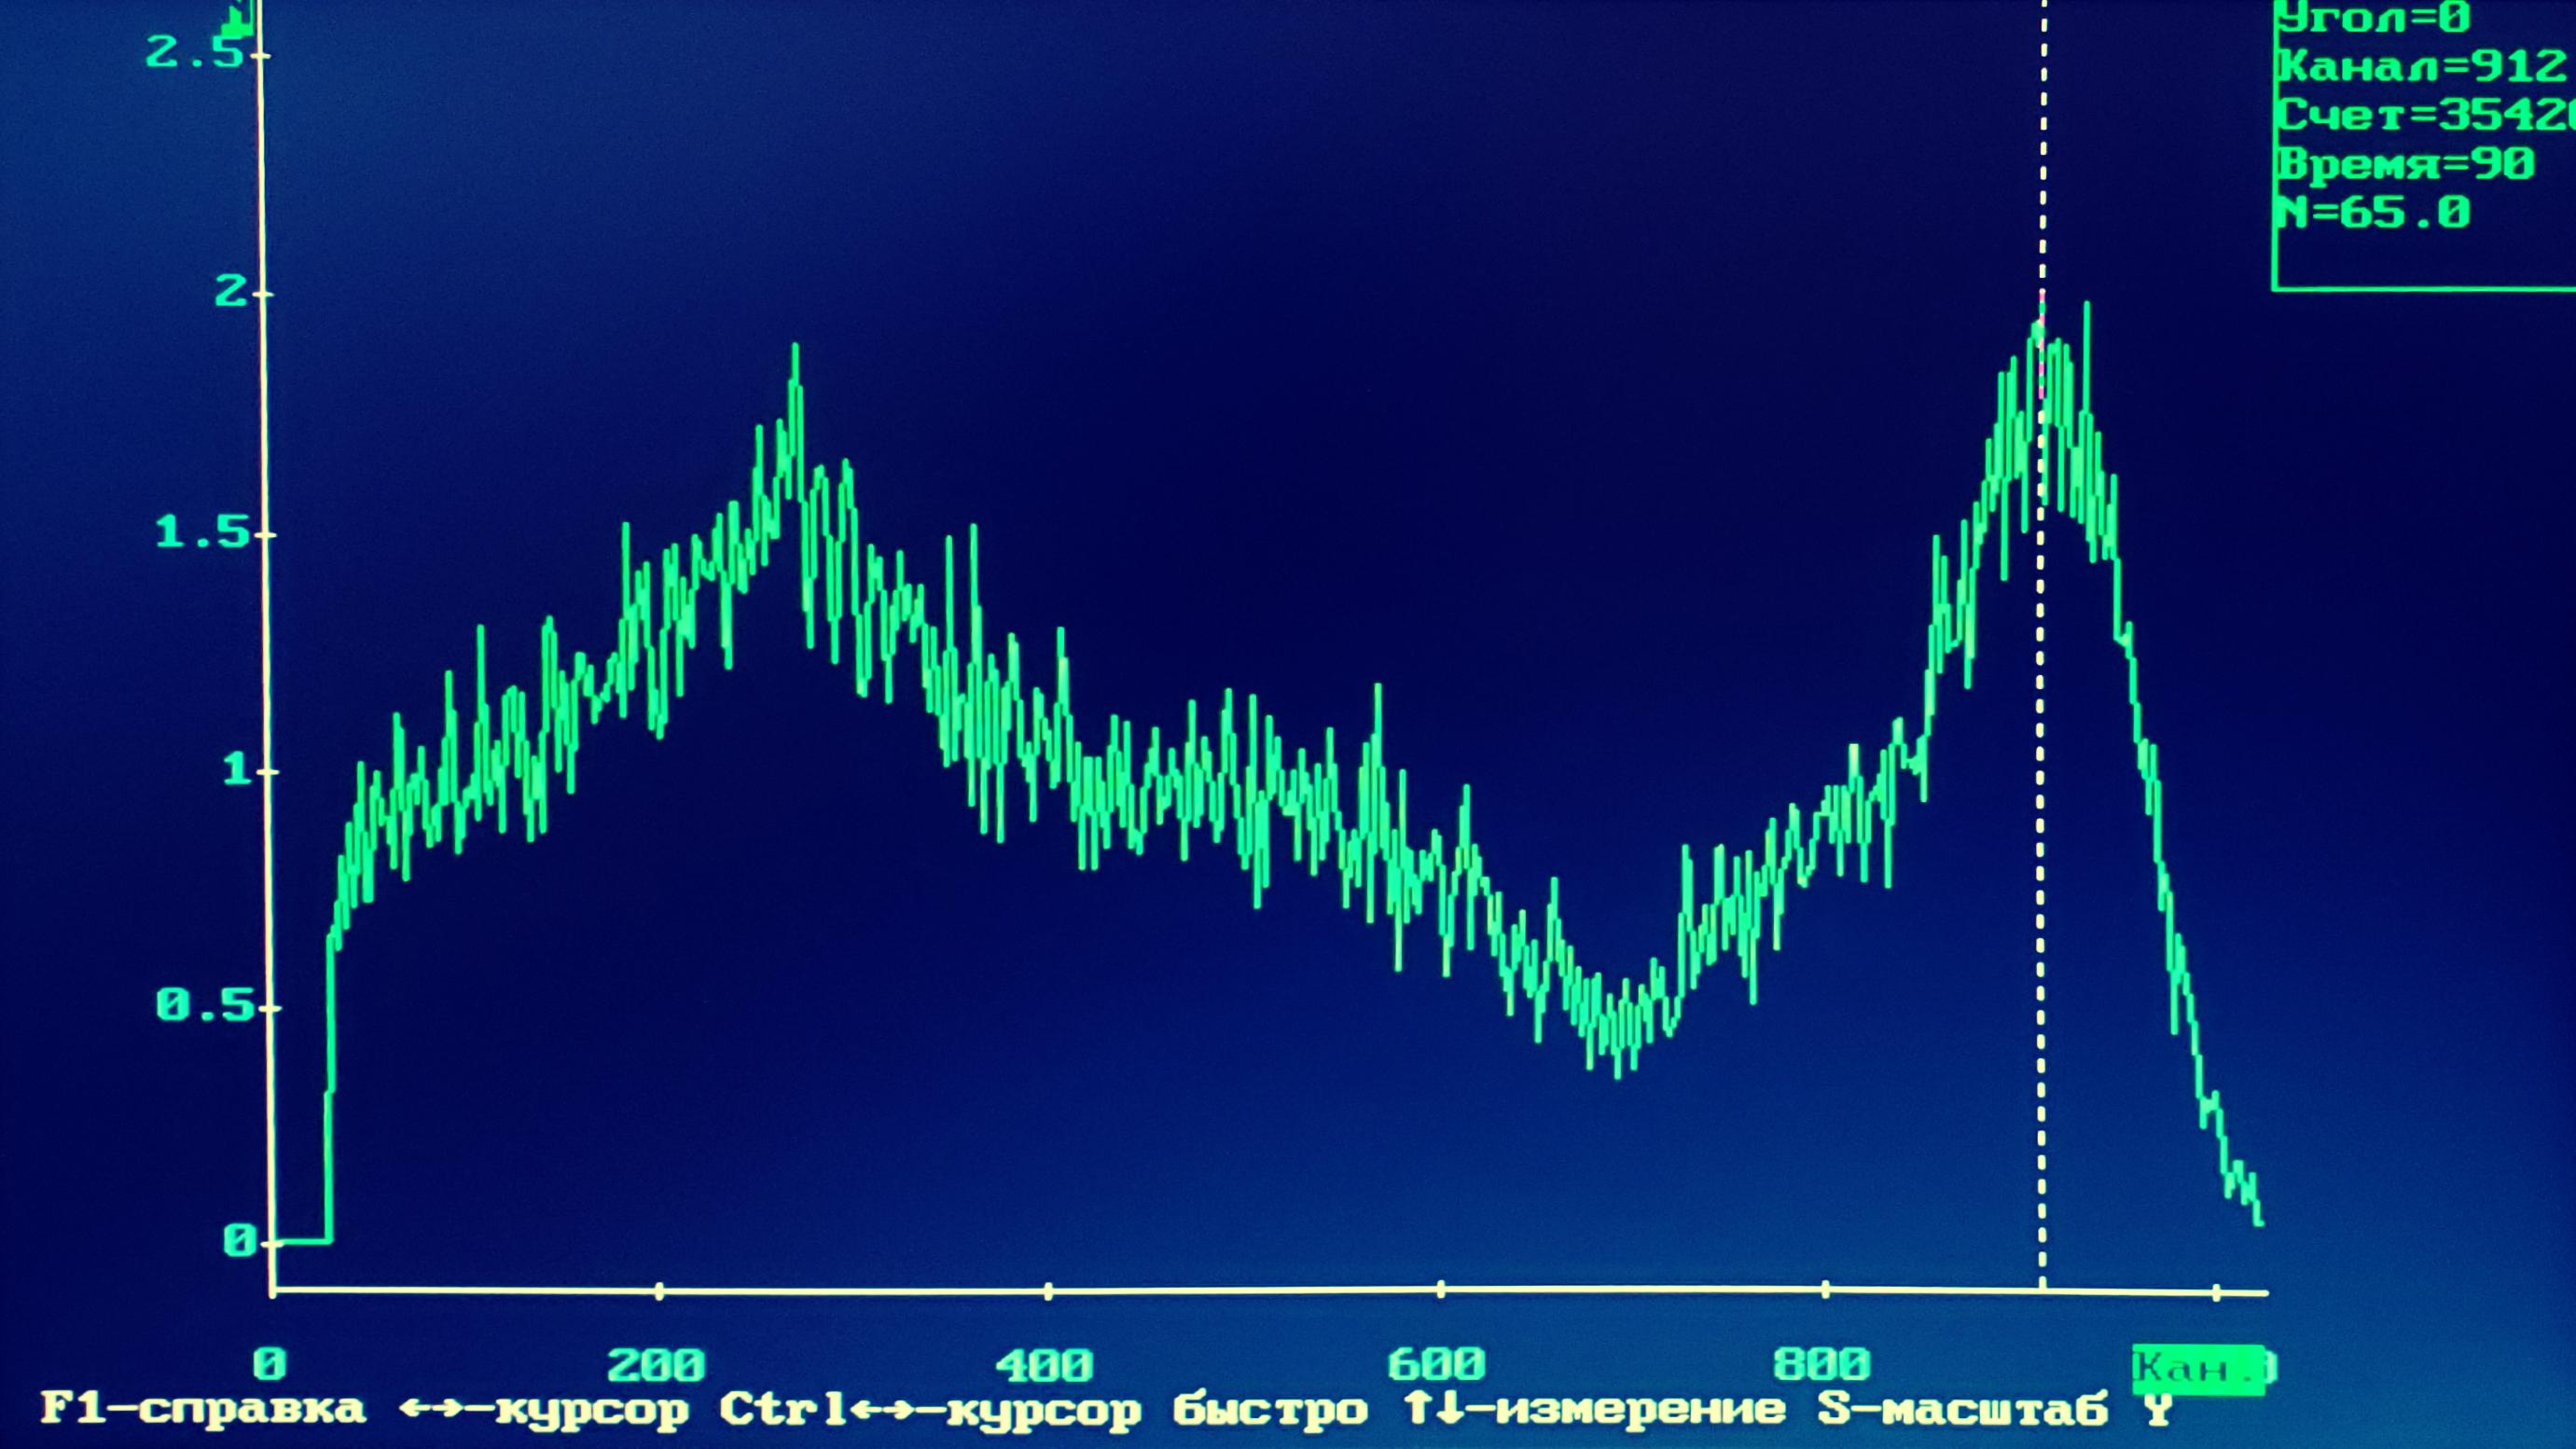
\includegraphics[width = \linewidth]{spectre0.jpg}}\\
      Рис 4. $\theta = 0^{\circ}$
    \end{minipage}
    \begin{minipage}[h]{0.32\linewidth}
      \center{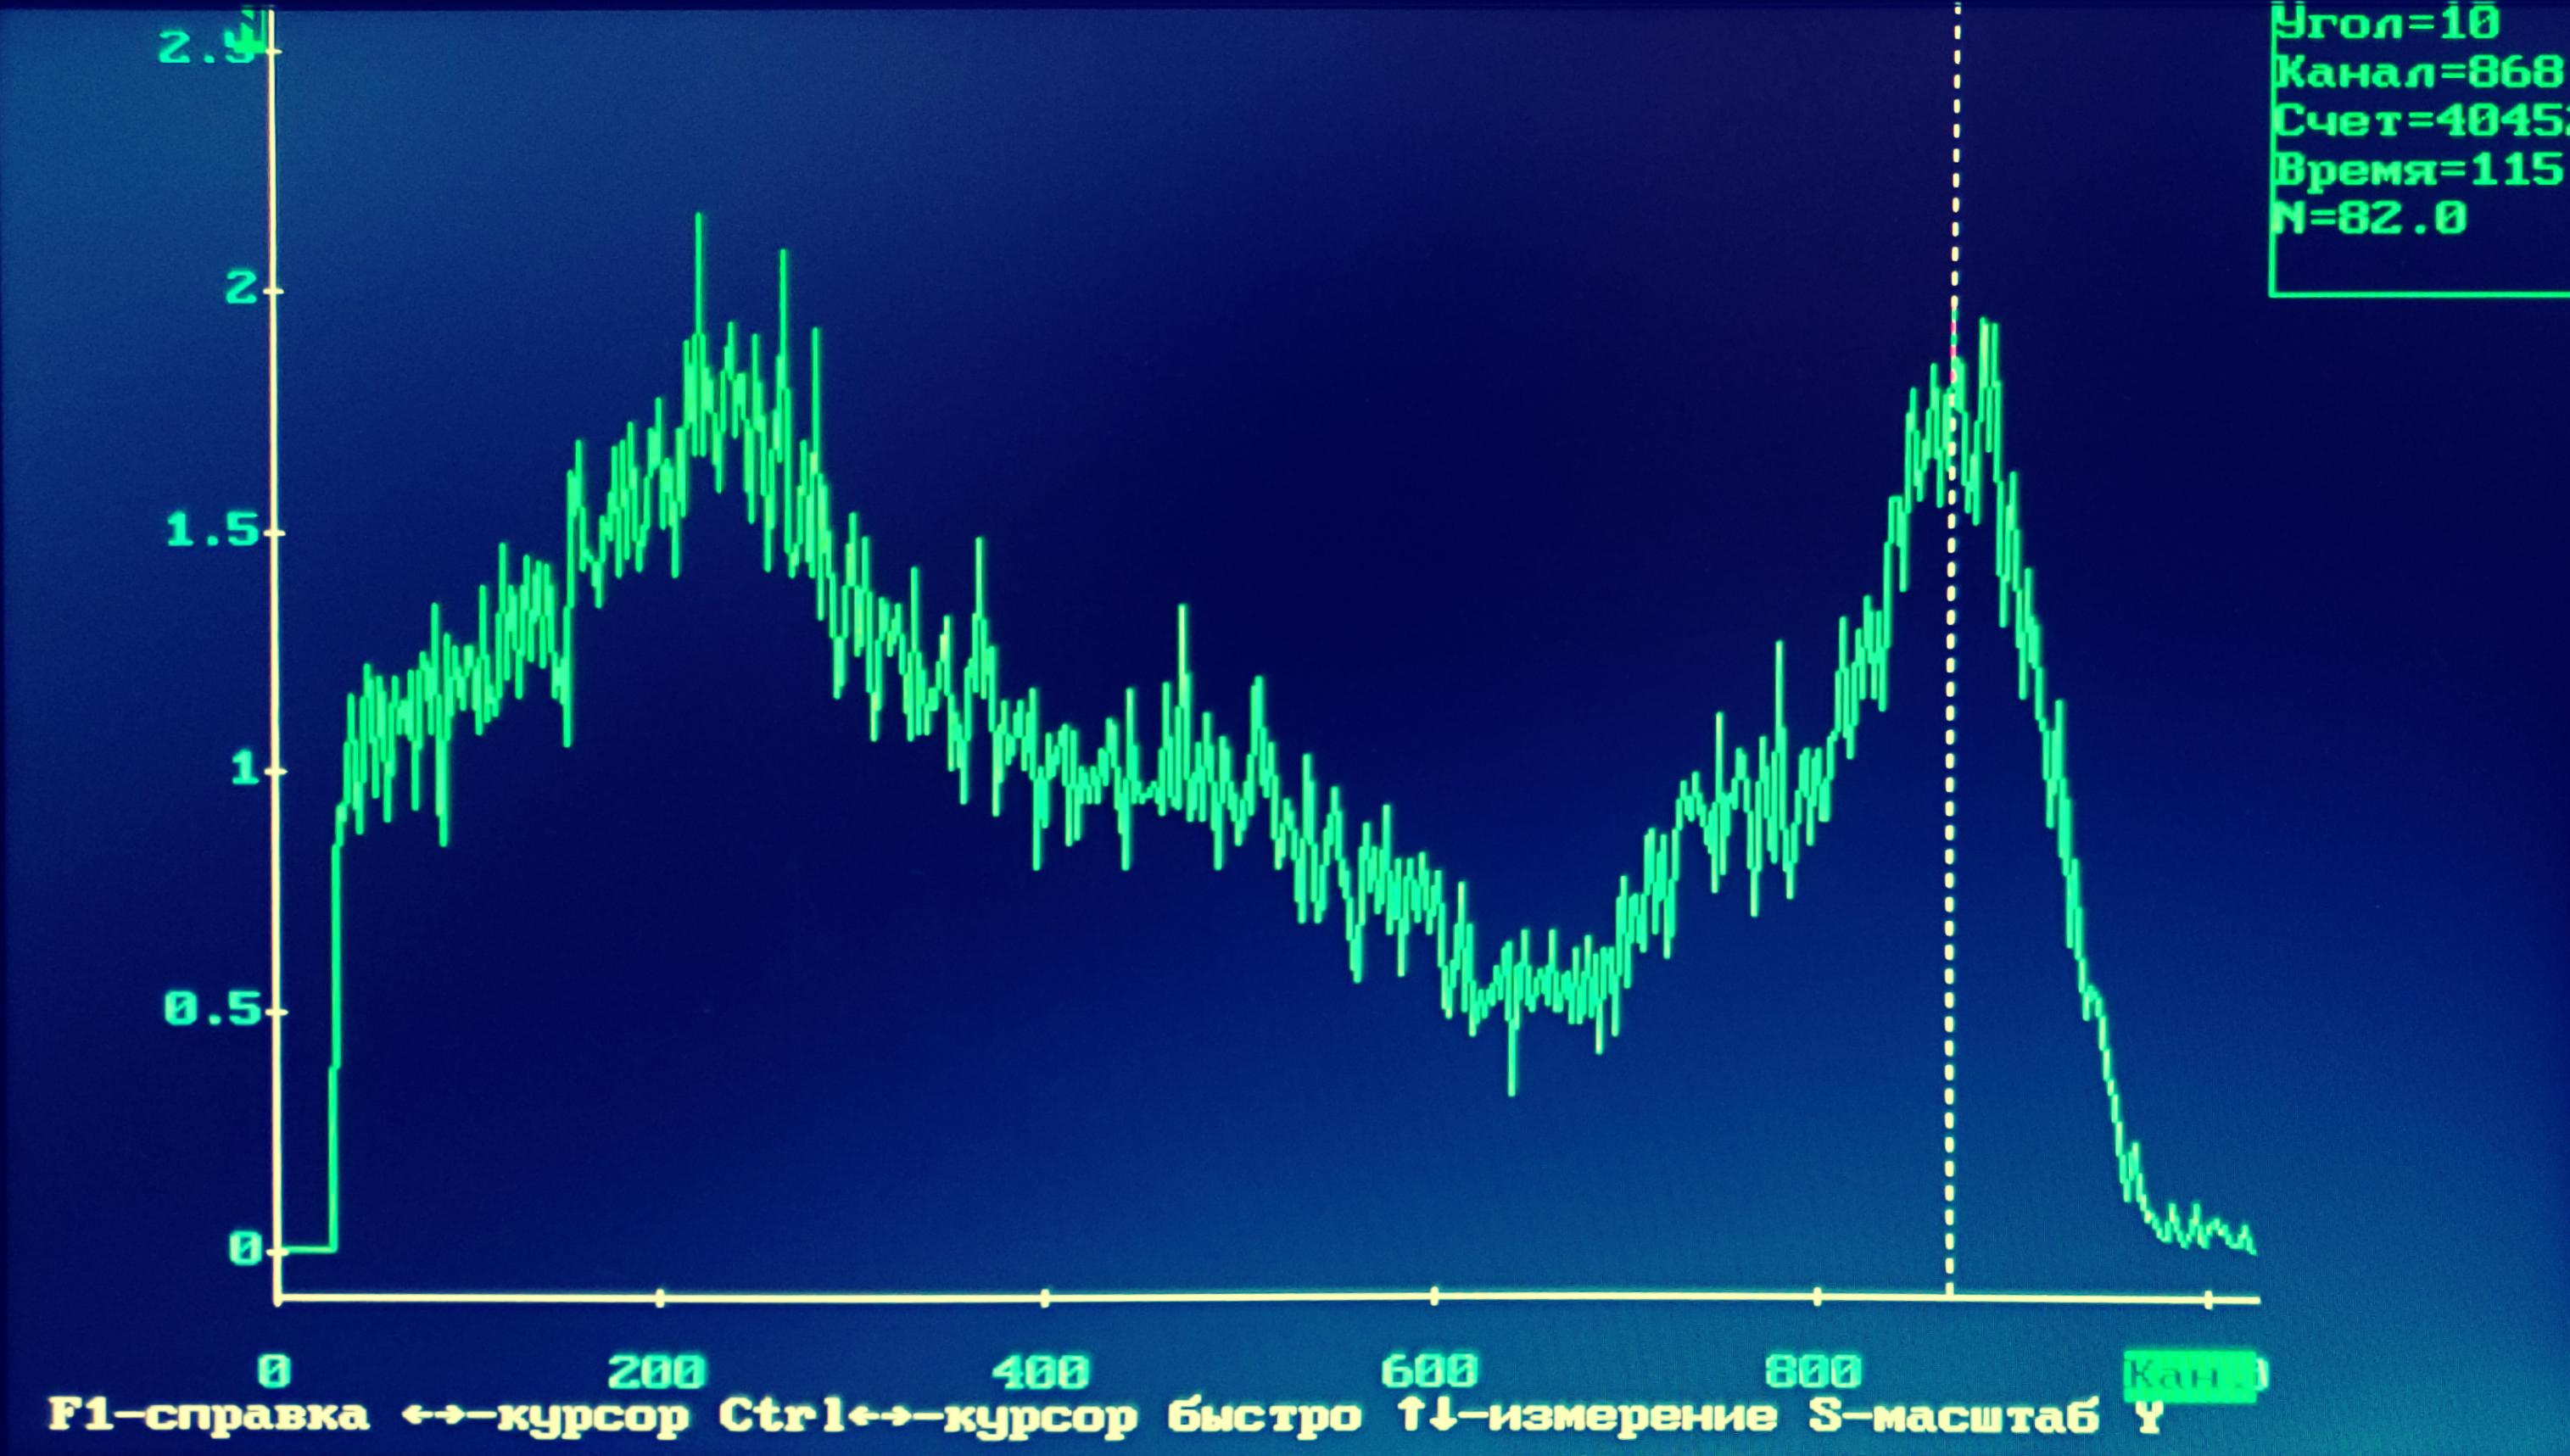
\includegraphics[width = \linewidth]{spectre10.jpg}}\\
      Рис 5. $\theta = 10^{\circ}$
    \end{minipage}
    \begin{minipage}[h]{0.32\linewidth}
      \center{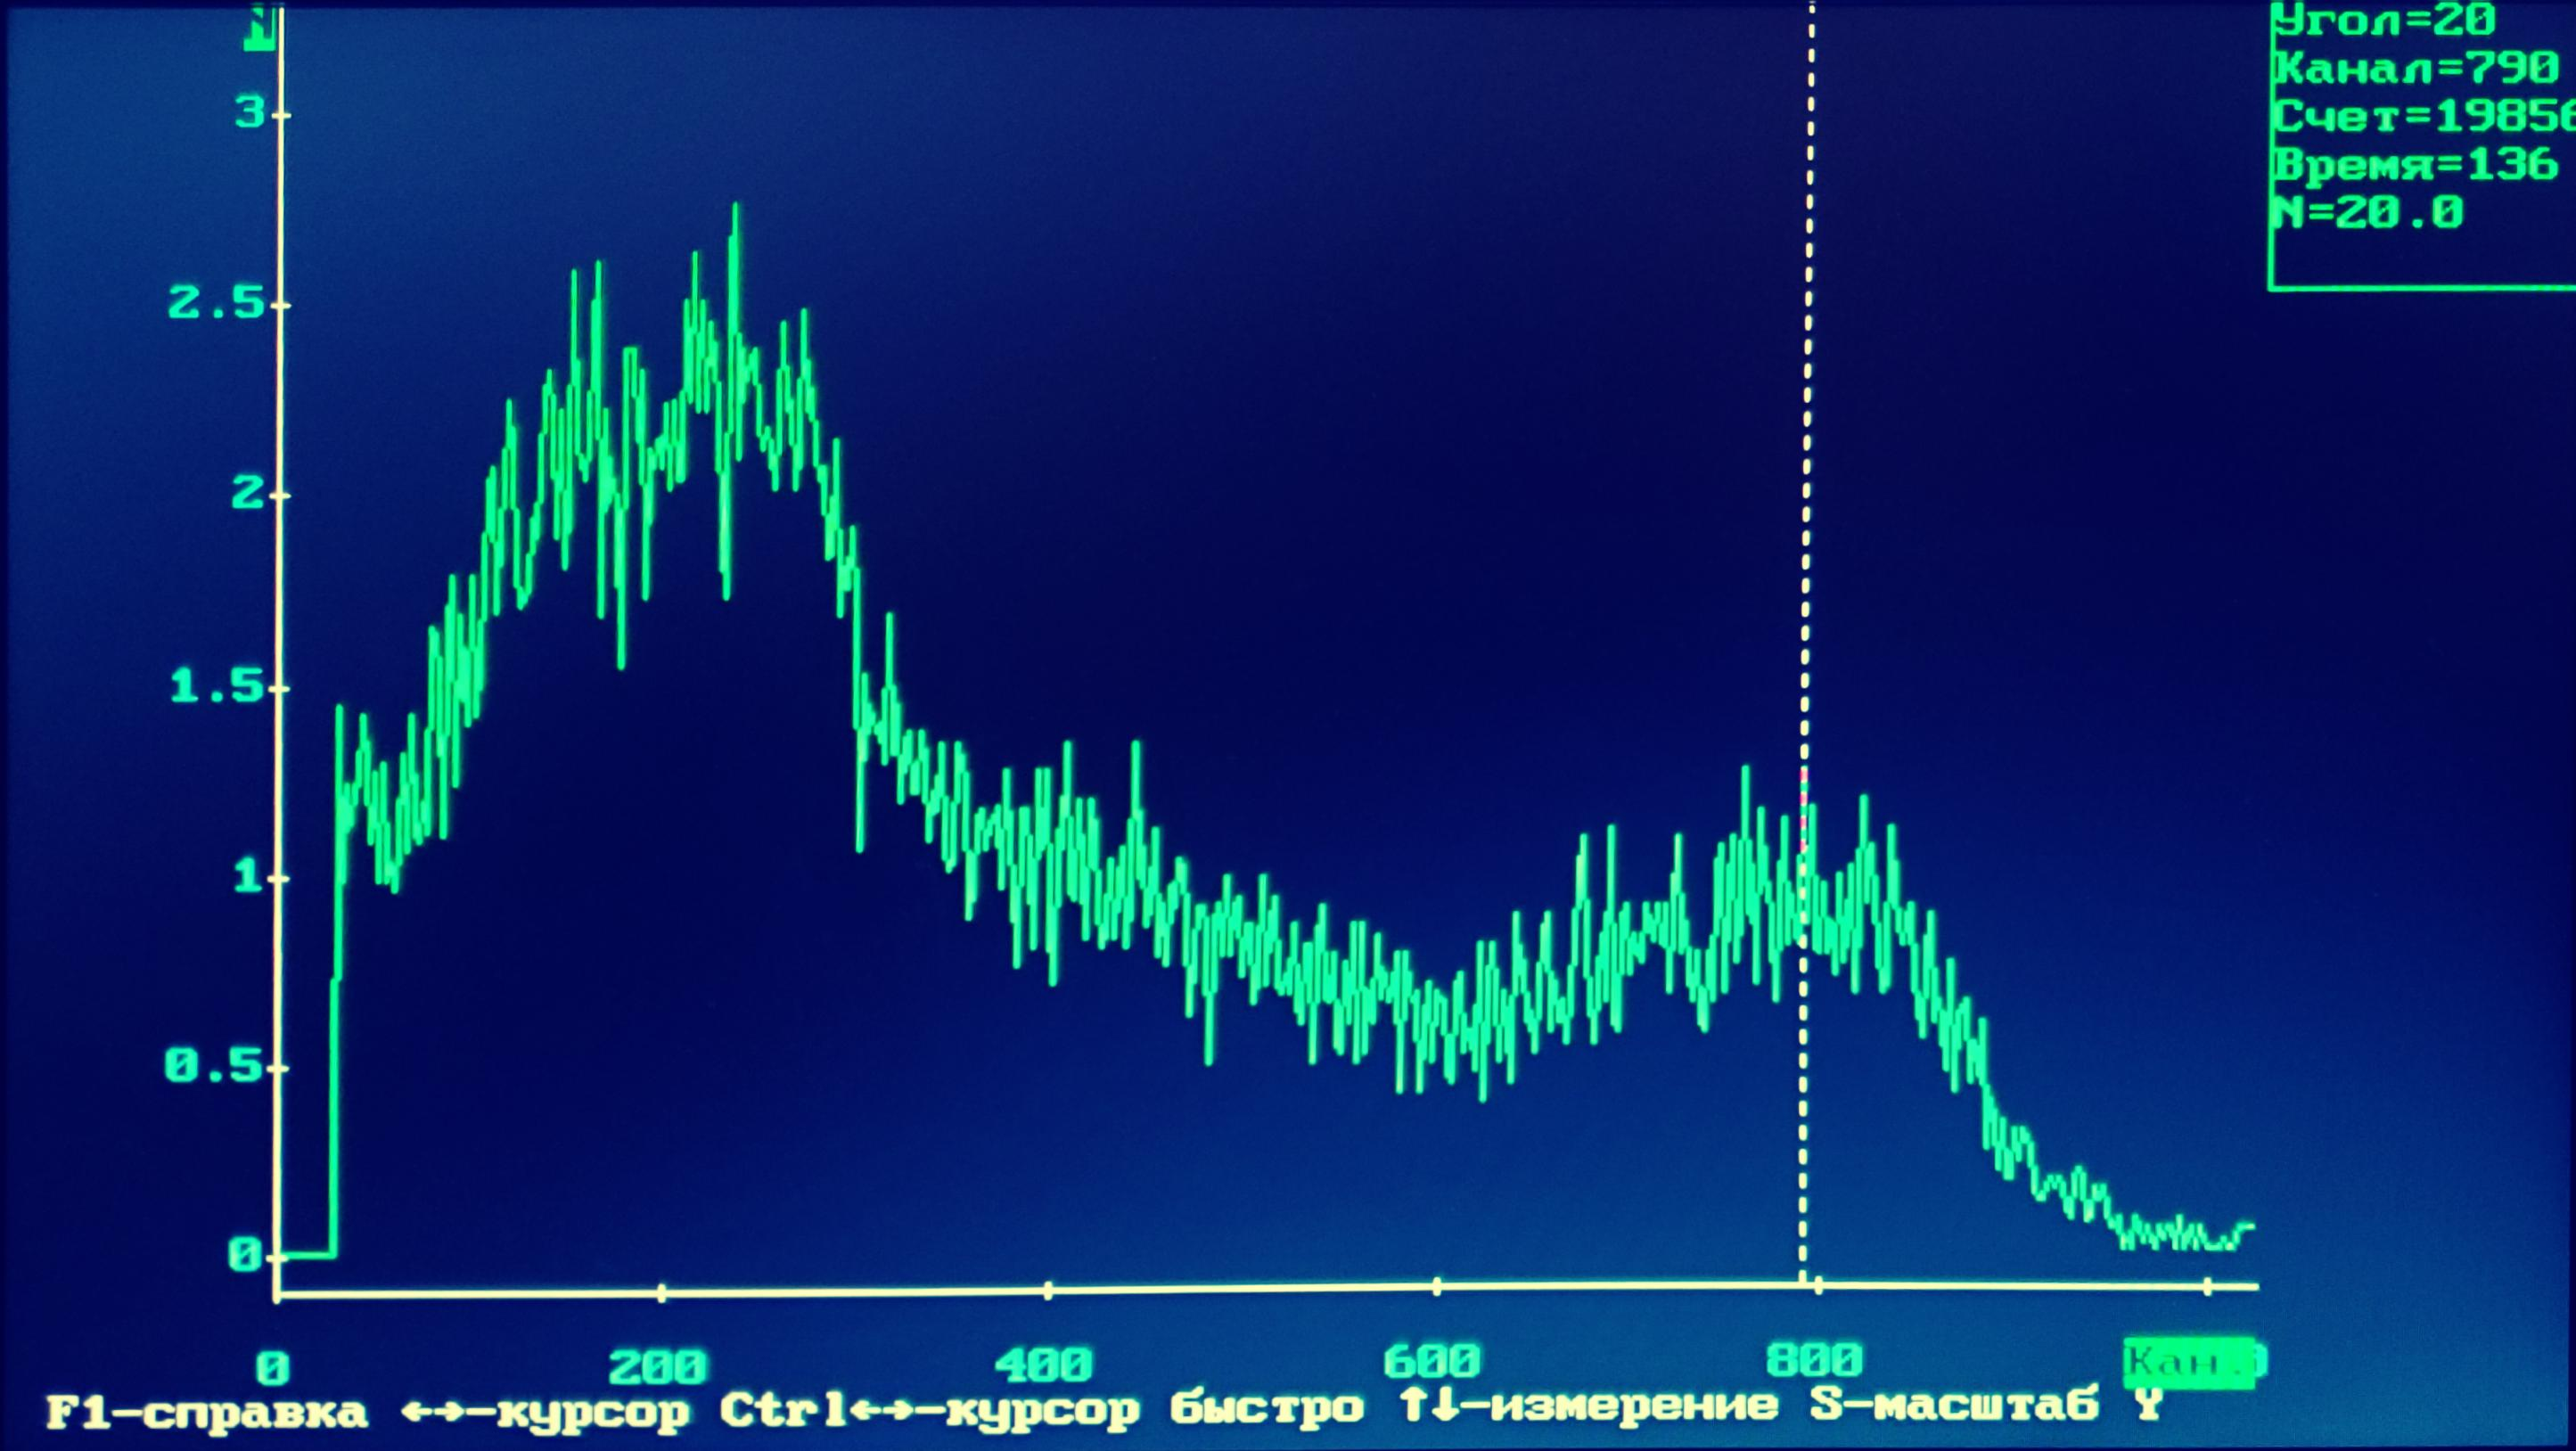
\includegraphics[width = \linewidth]{spectre20.jpg}}\\
      Рис 6. $\theta = 20^{\circ}$
    \end{minipage}
  \end{figure}
  \begin{figure}[h!]
    \begin{minipage}[h]{0.32\linewidth}
      \center{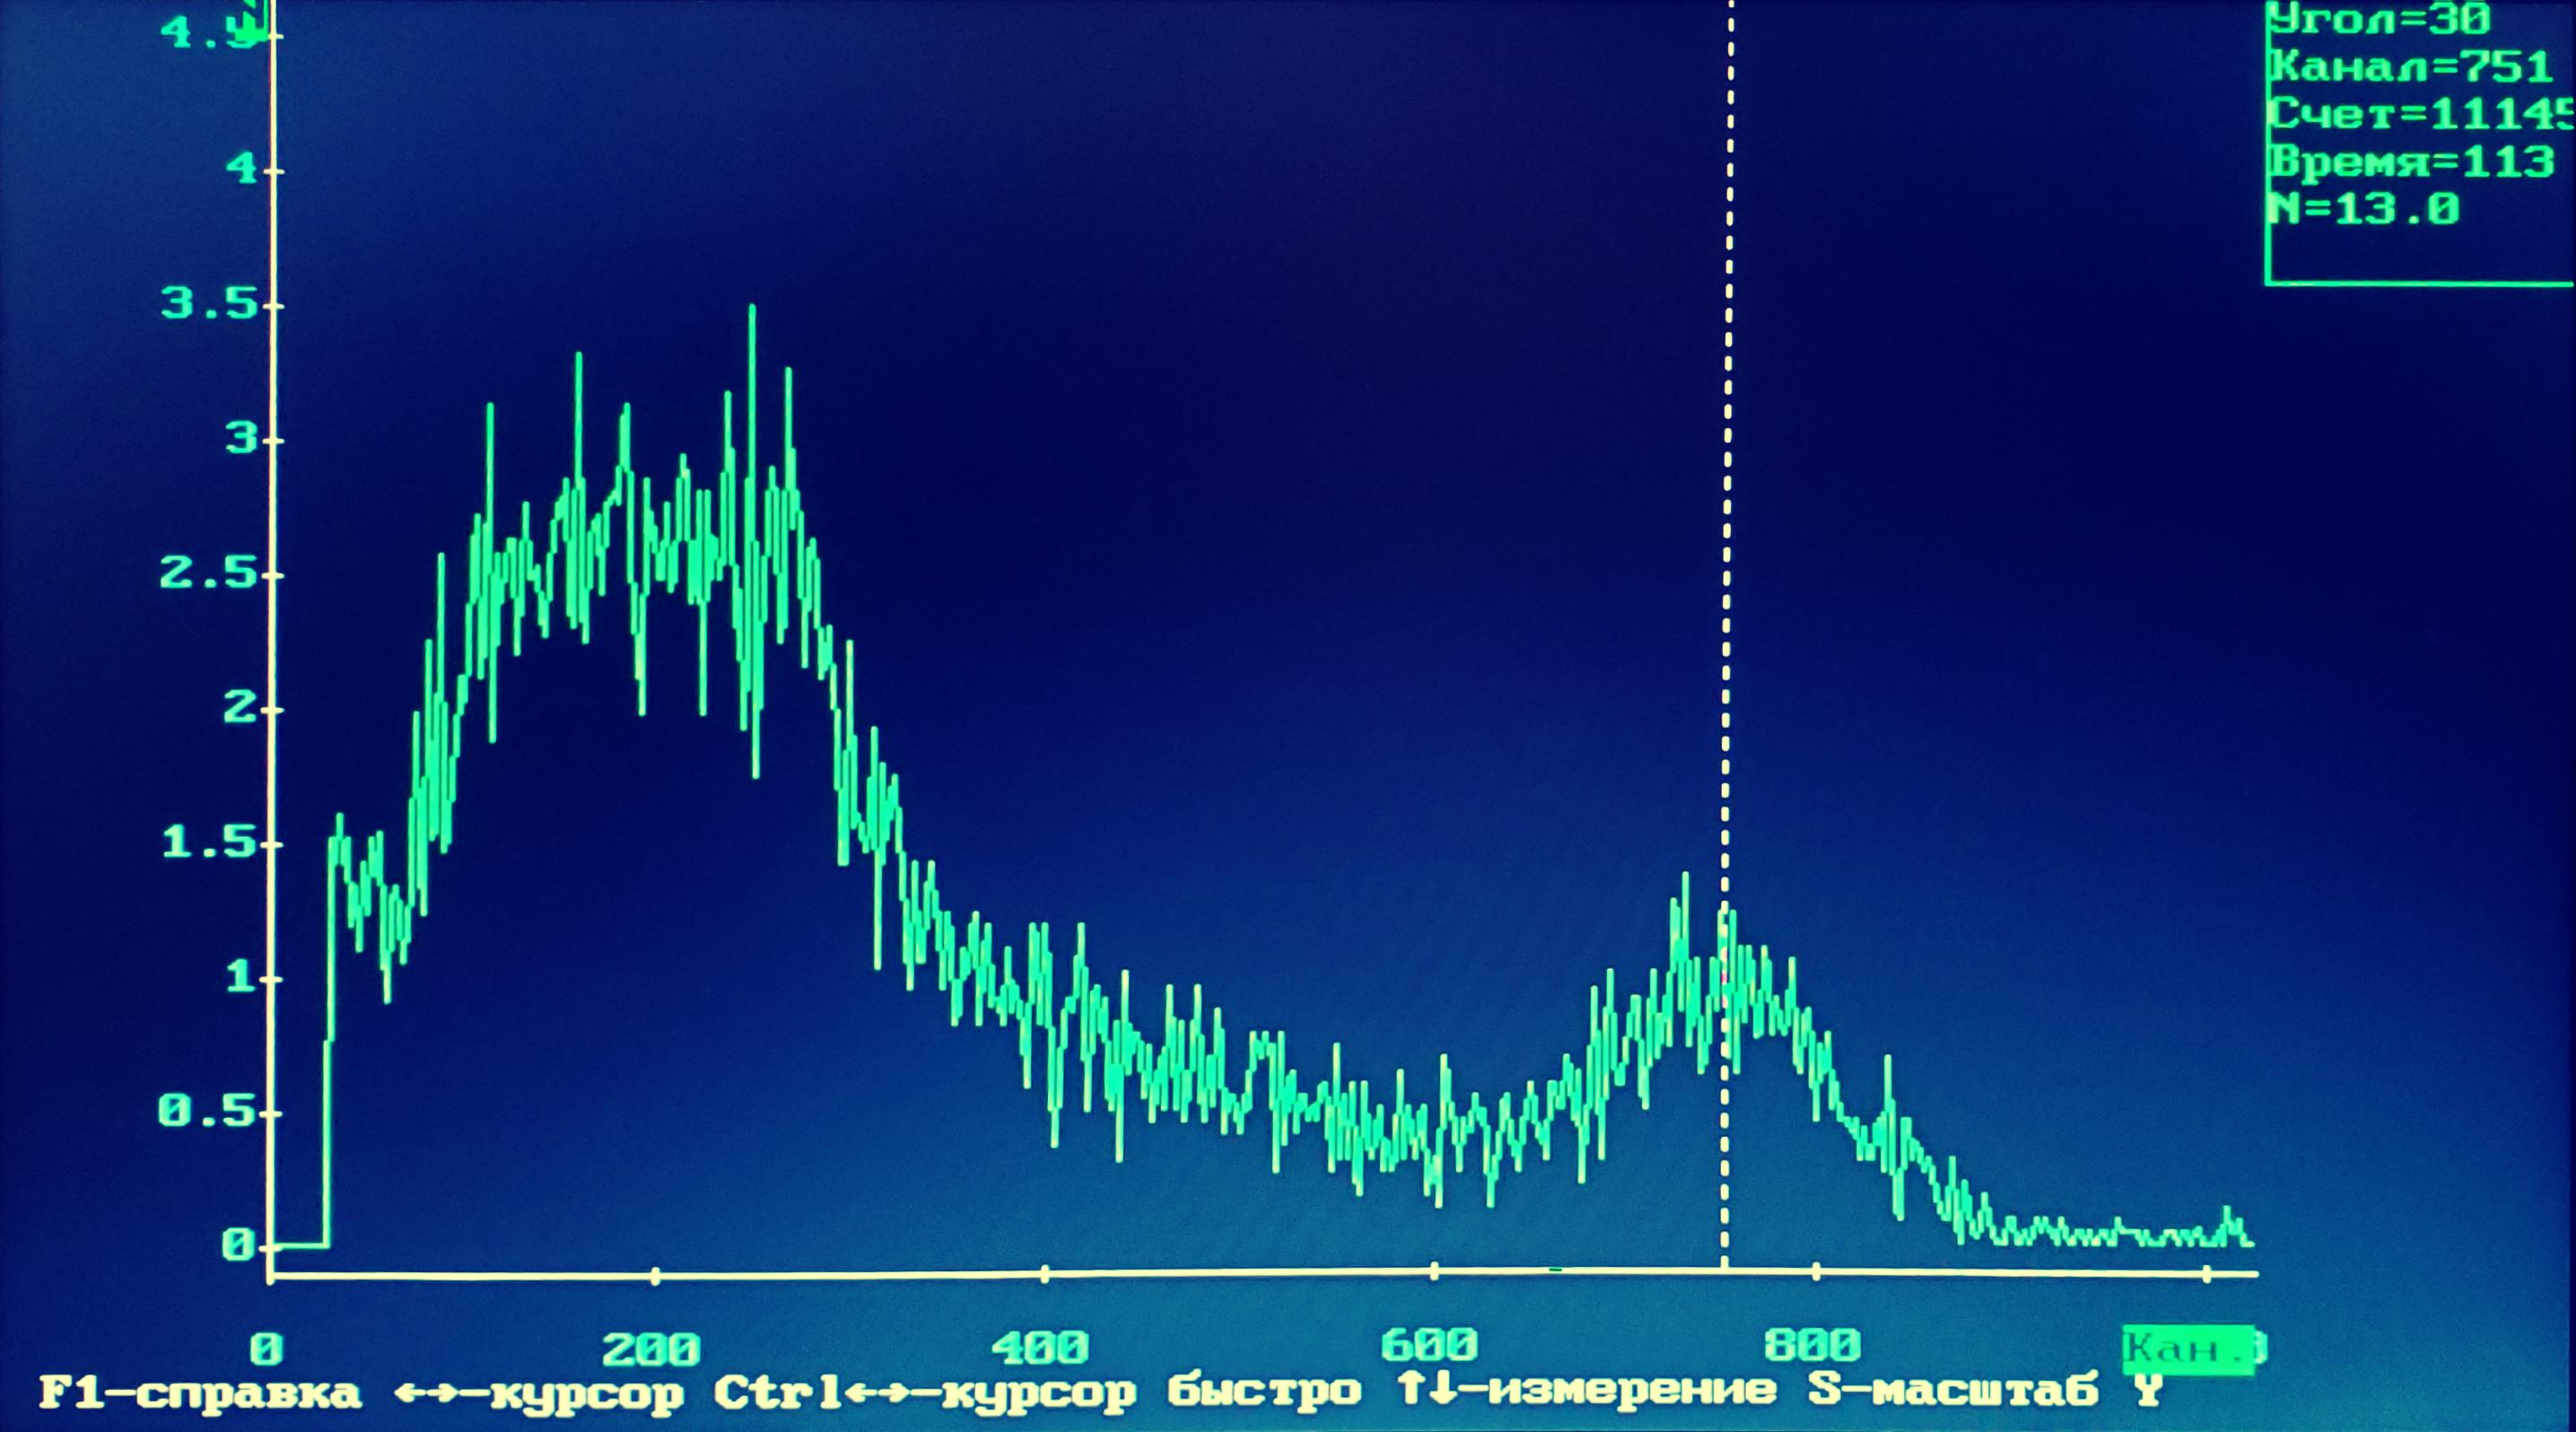
\includegraphics[width = \linewidth]{spectre30.jpg}}\\
      Рис 7. $\theta = 30^{\circ}$
    \end{minipage}
    \begin{minipage}[h]{0.32\linewidth}
      \center{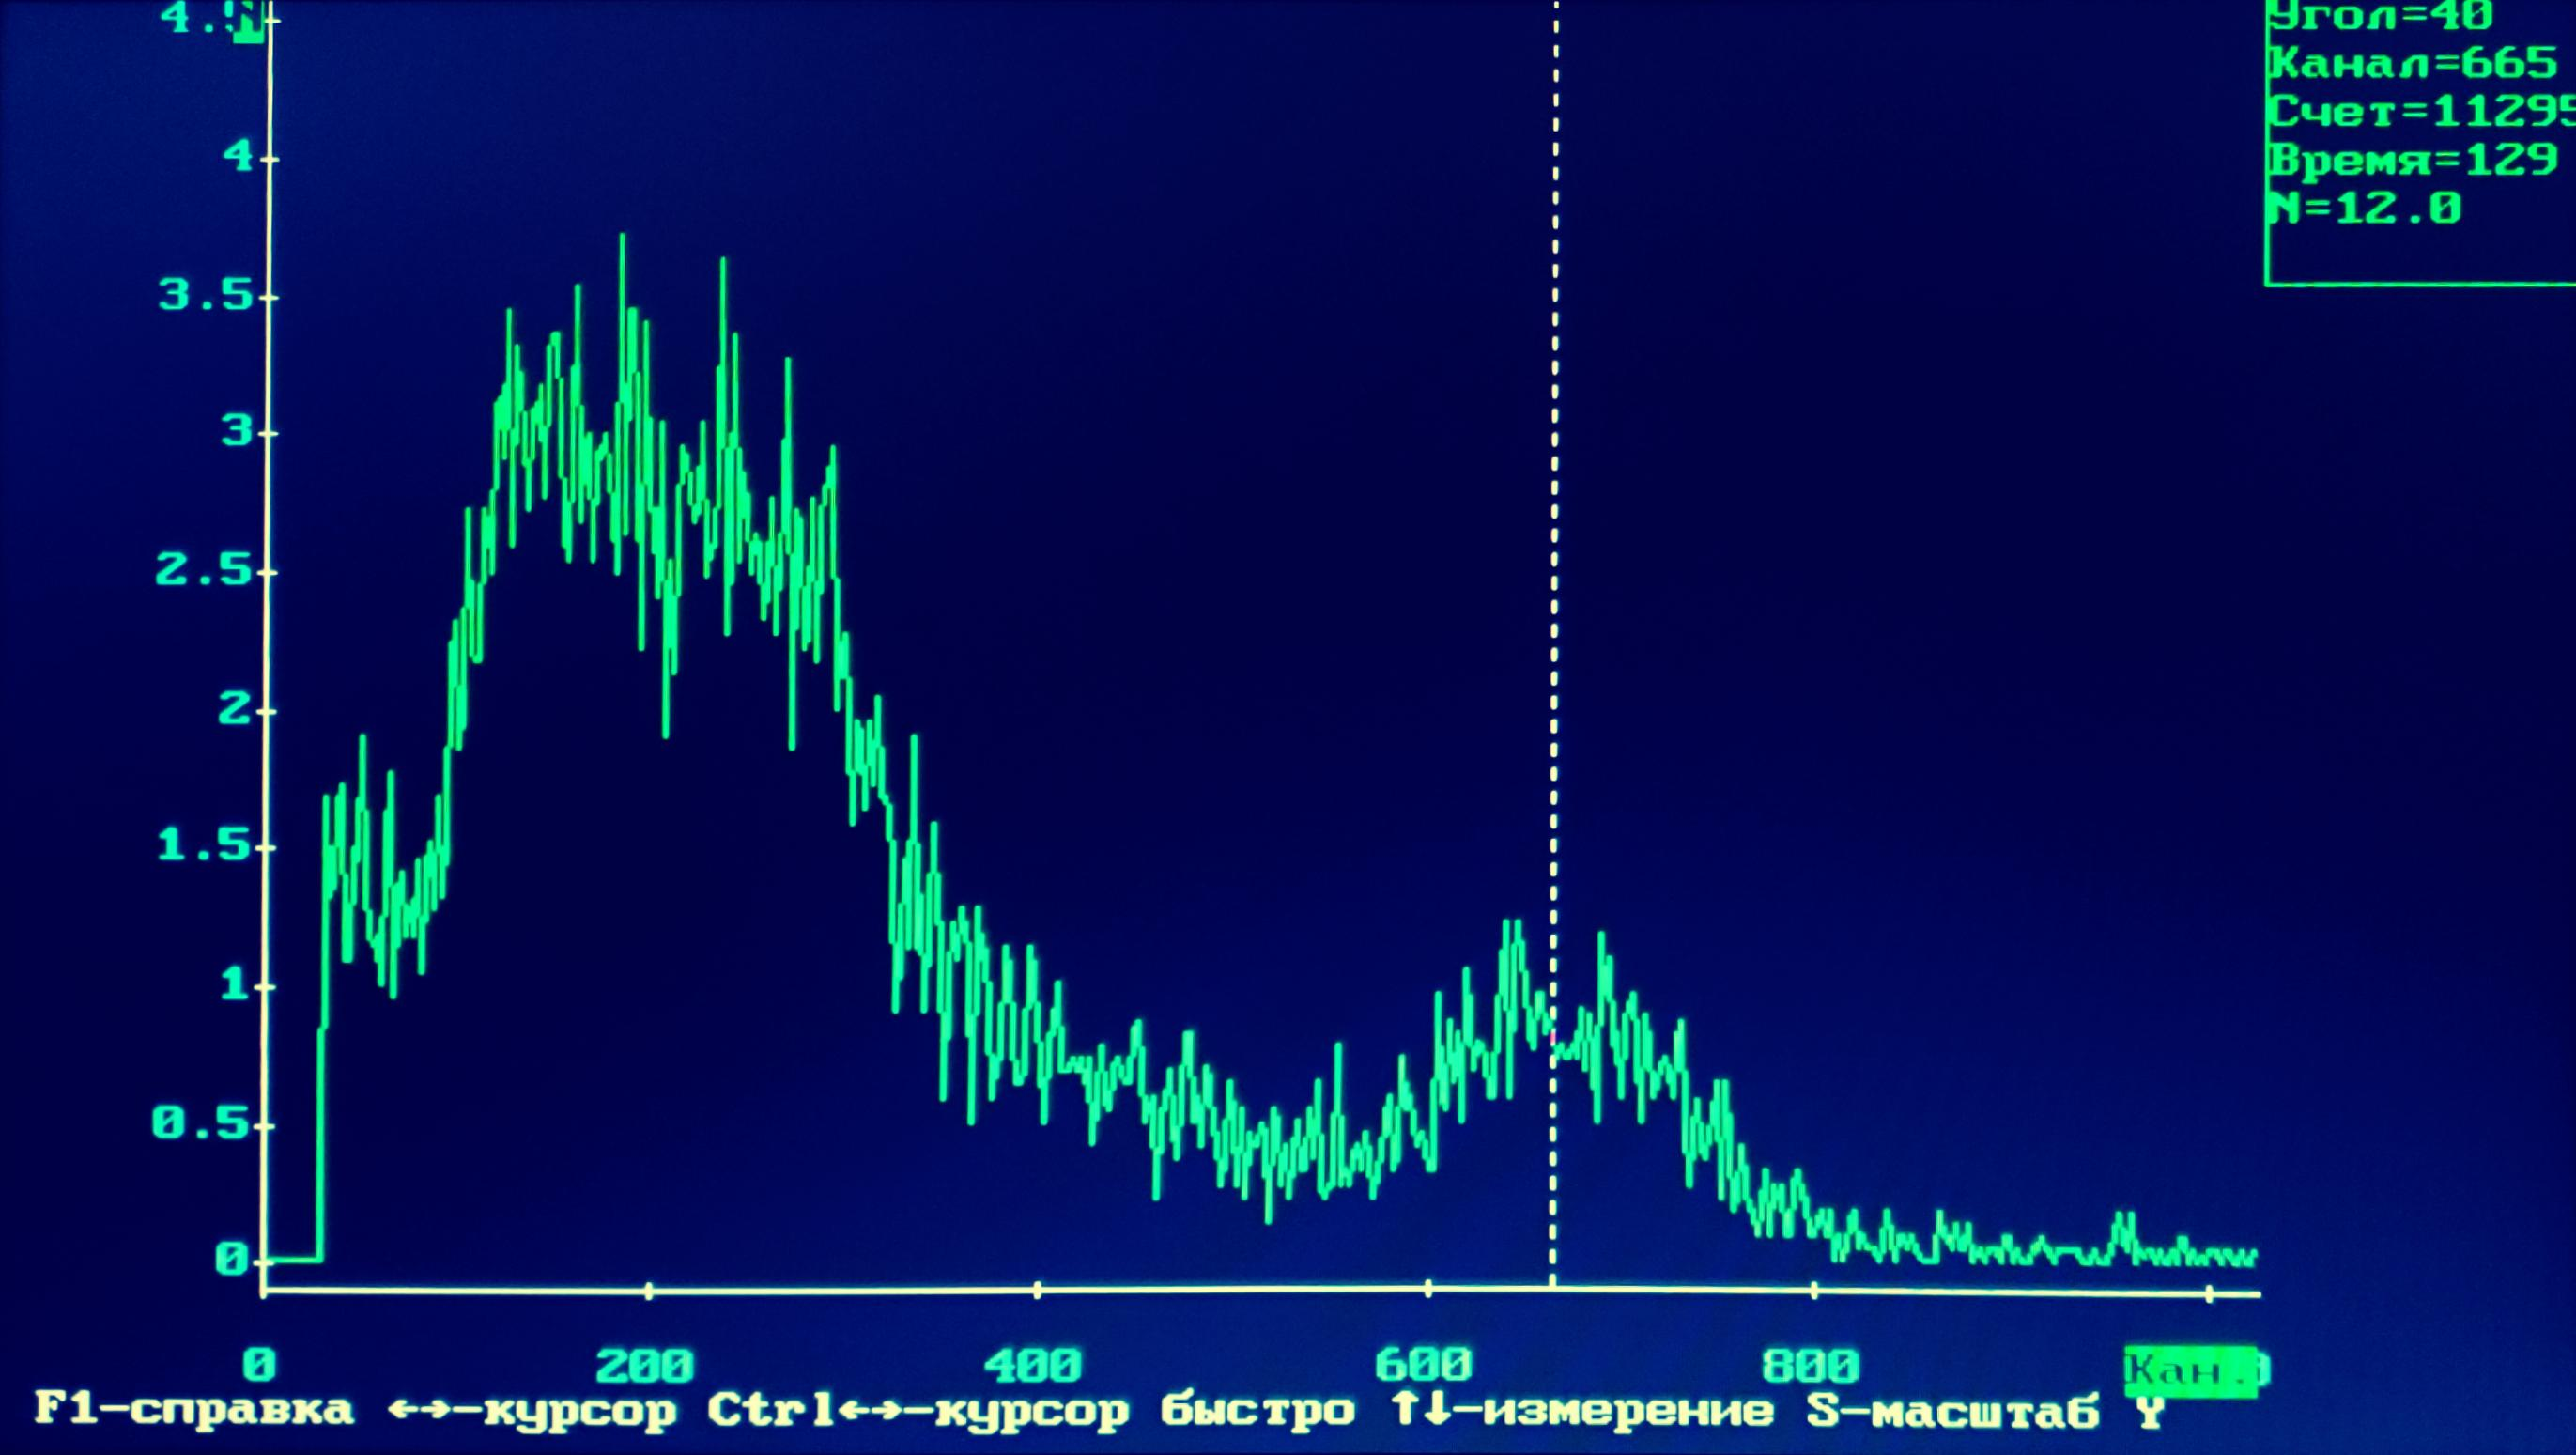
\includegraphics[width = \linewidth]{spectre40.jpg}}\\
      Рис 8. $\theta = 40^{\circ}$
    \end{minipage}
    \begin{minipage}[h]{0.32\linewidth}
      \center{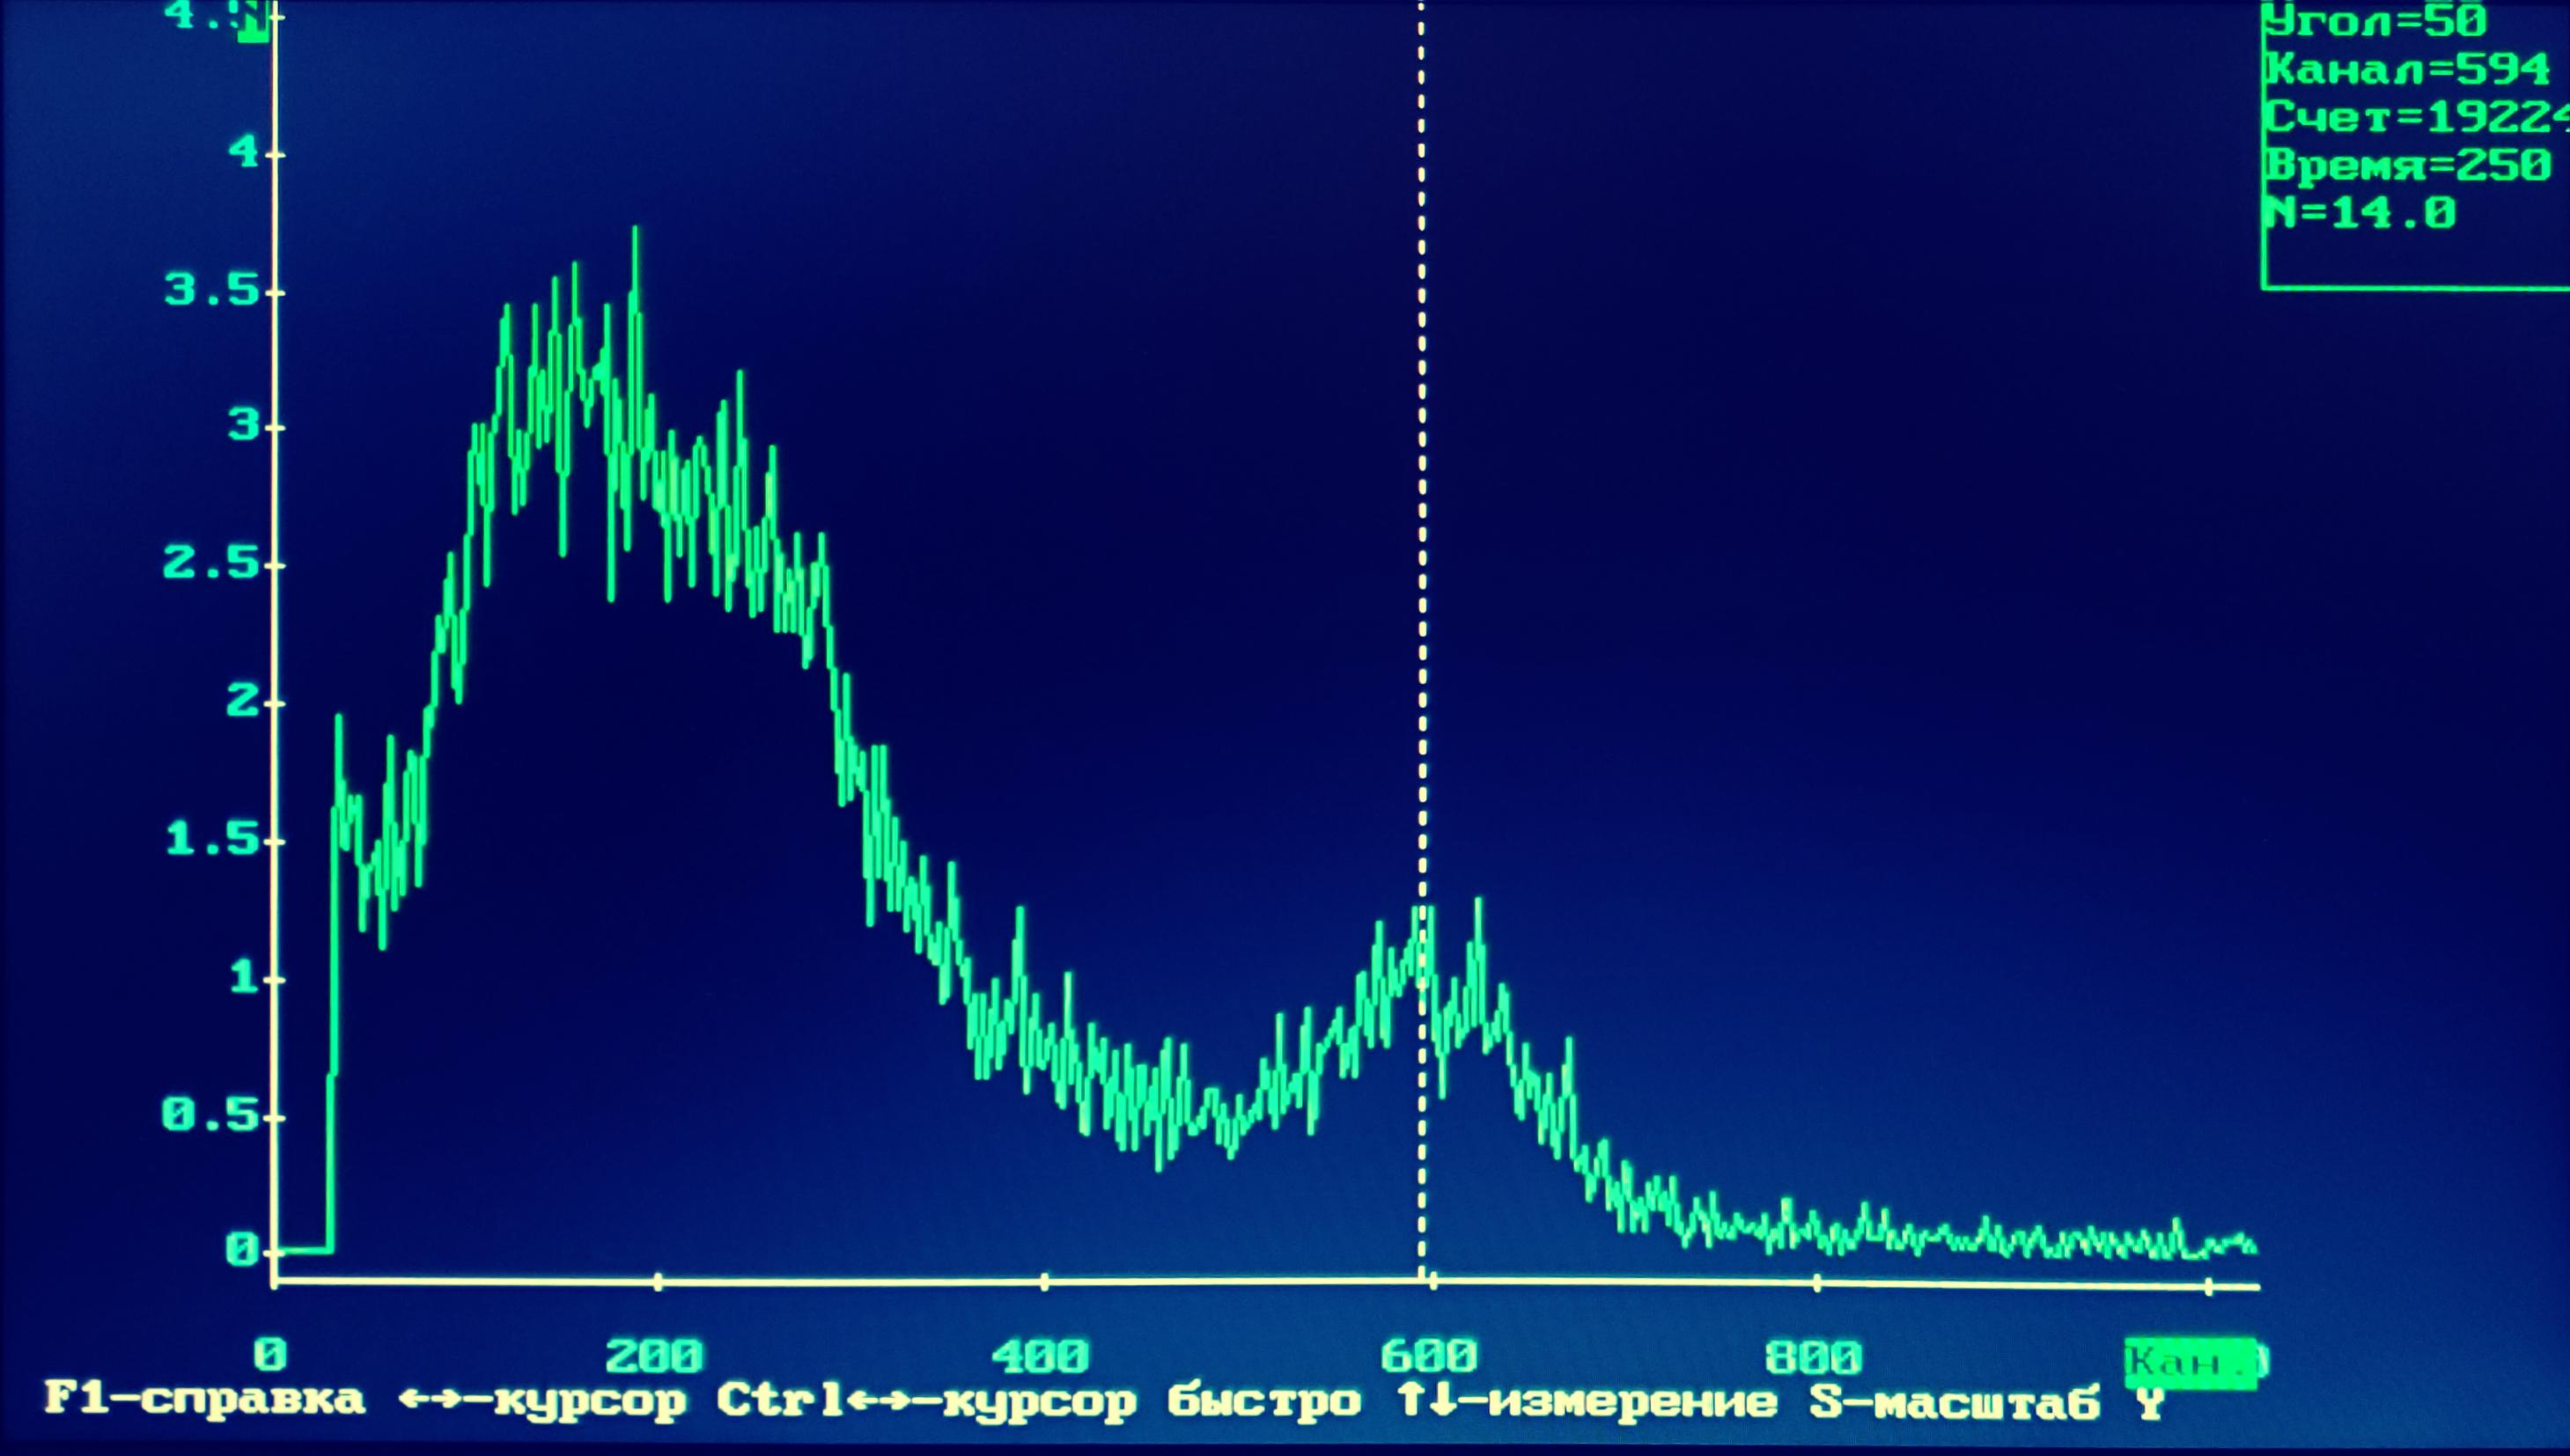
\includegraphics[width = \linewidth]{spectre50.jpg}}\\
      Рис 9. $\theta = 50^{\circ}$
    \end{minipage}
  \end{figure}
  \begin{figure}[h!]
    \begin{minipage}[h]{0.32\linewidth}
      \center{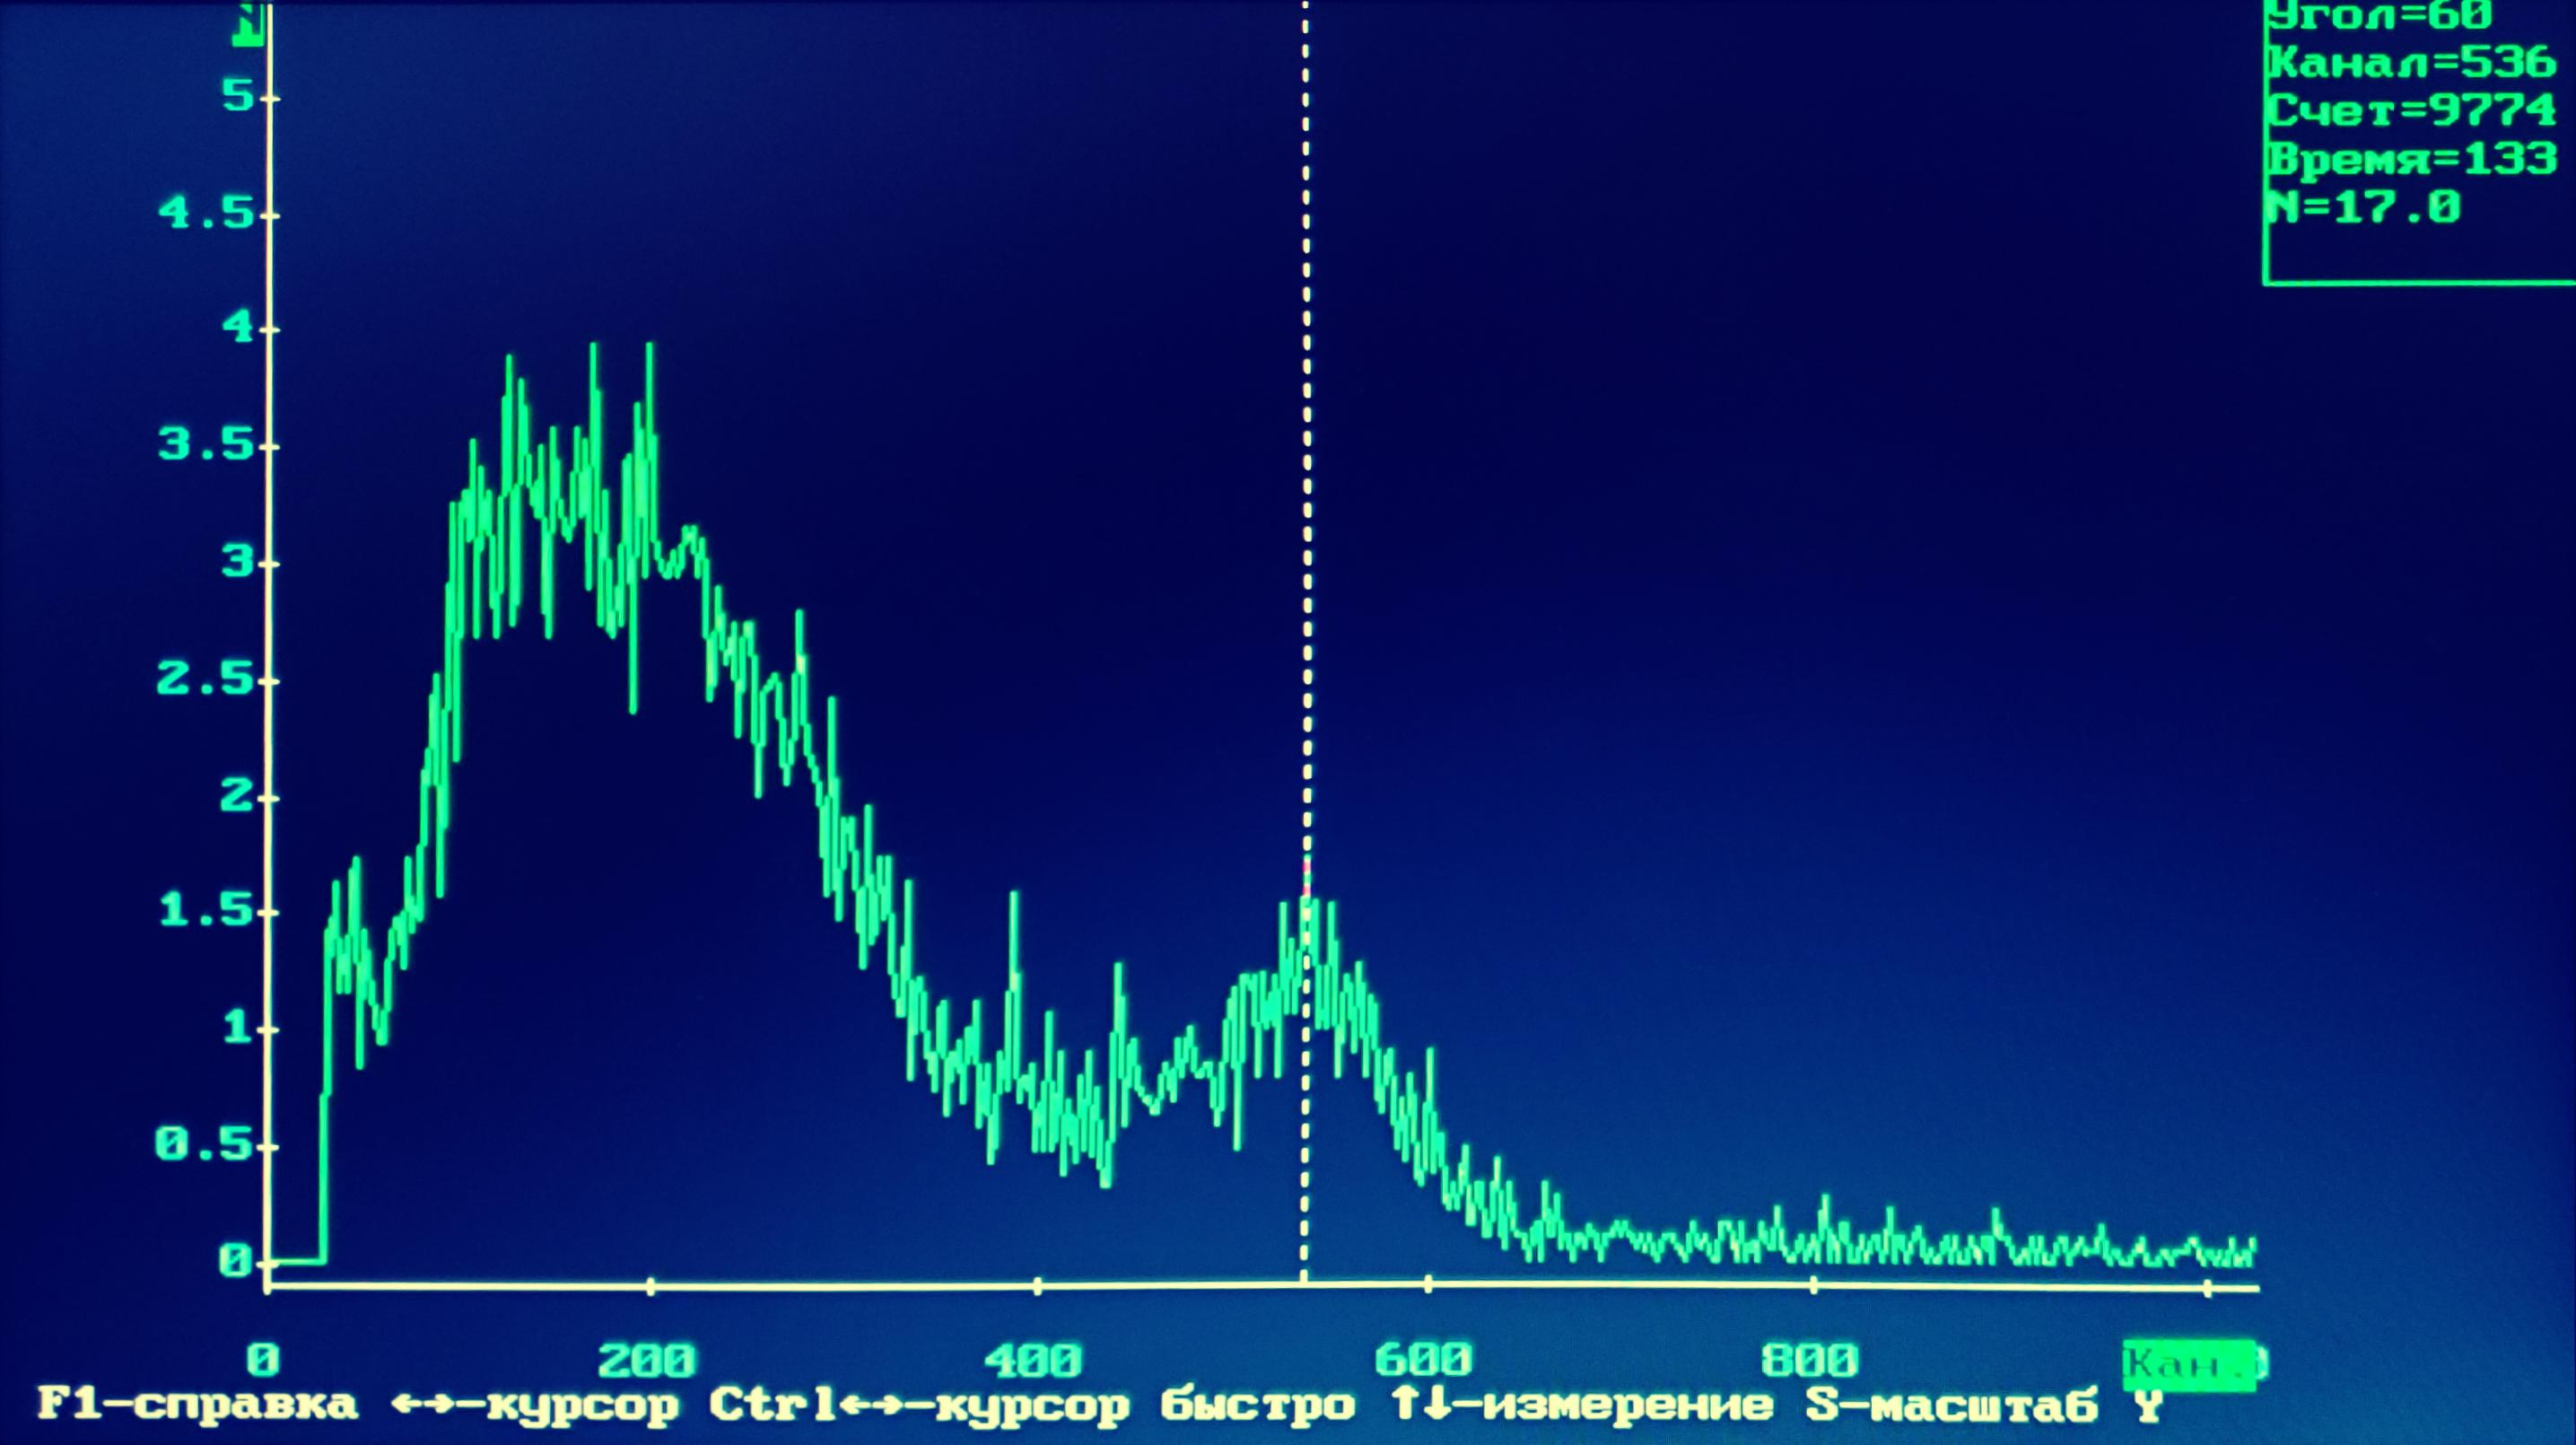
\includegraphics[width = \linewidth]{spectre60.jpg}}\\
      Рис 10. $\theta = 60^{\circ}$
    \end{minipage}
    \begin{minipage}[h]{0.32\linewidth}
      \center{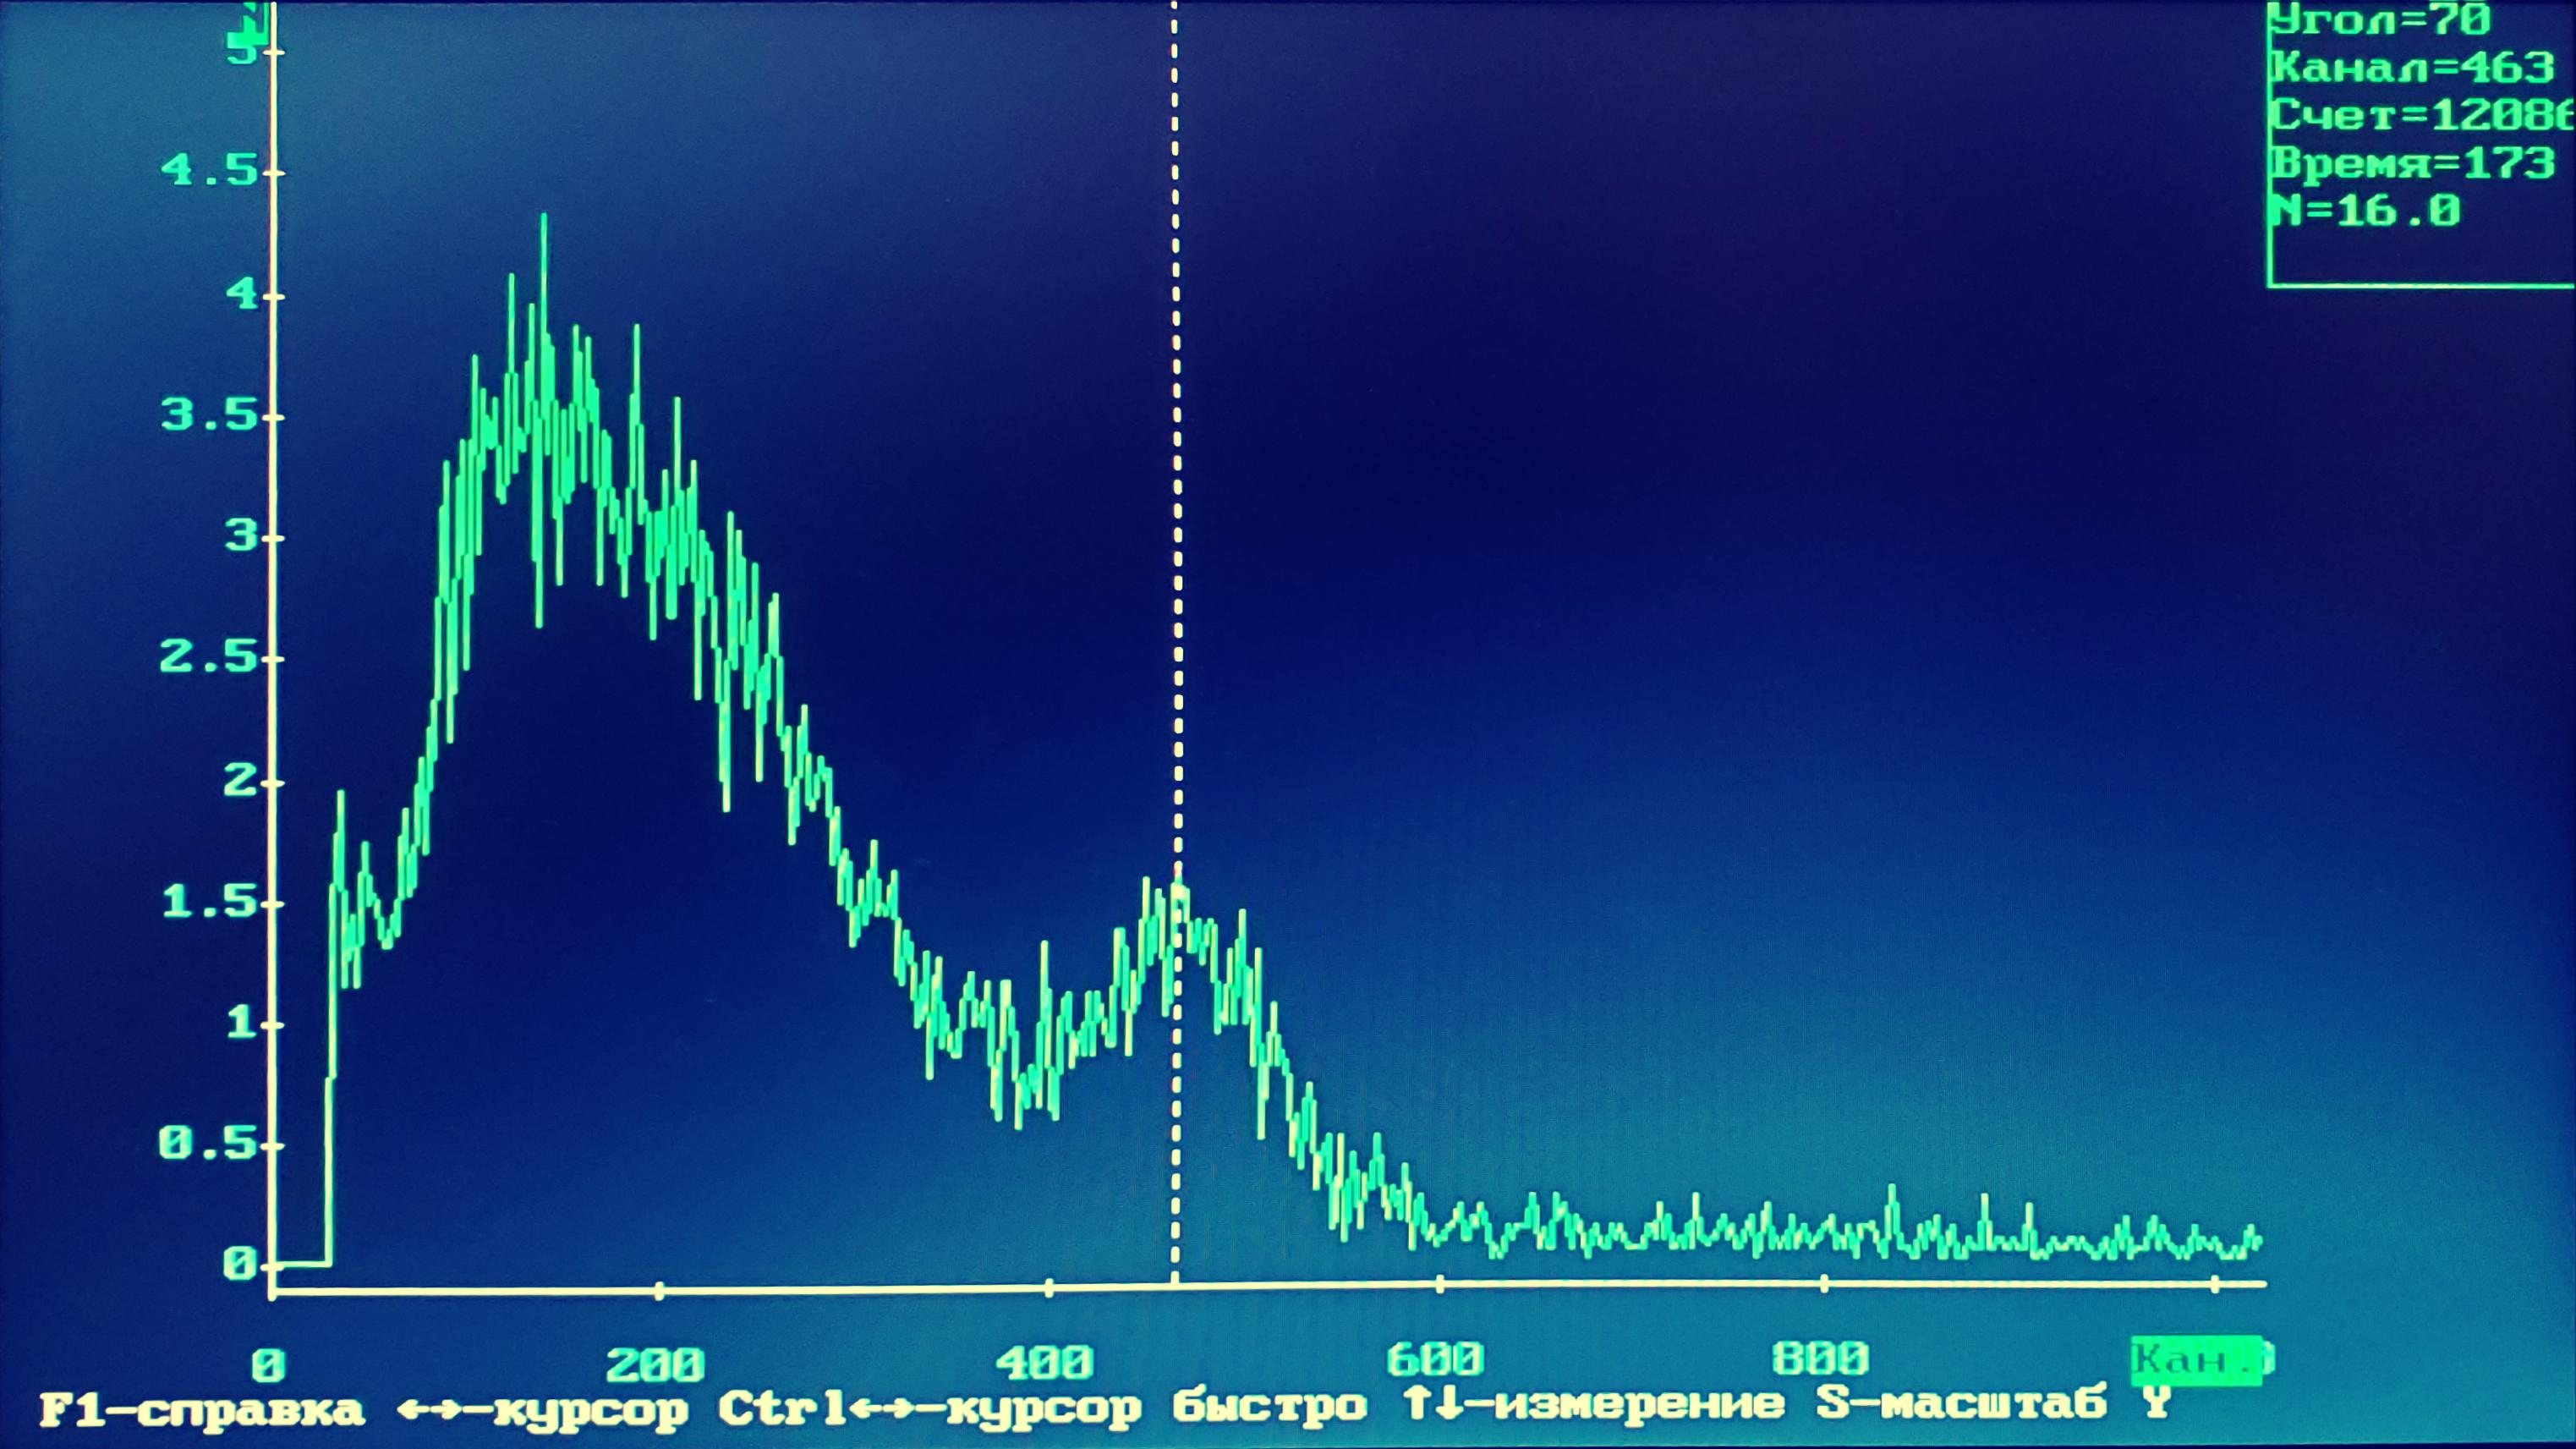
\includegraphics[width = \linewidth]{spectre70.jpg}}\\
      Рис 11. $\theta = 70^{\circ}$
    \end{minipage}
    \begin{minipage}[h]{0.32\linewidth}
      \center{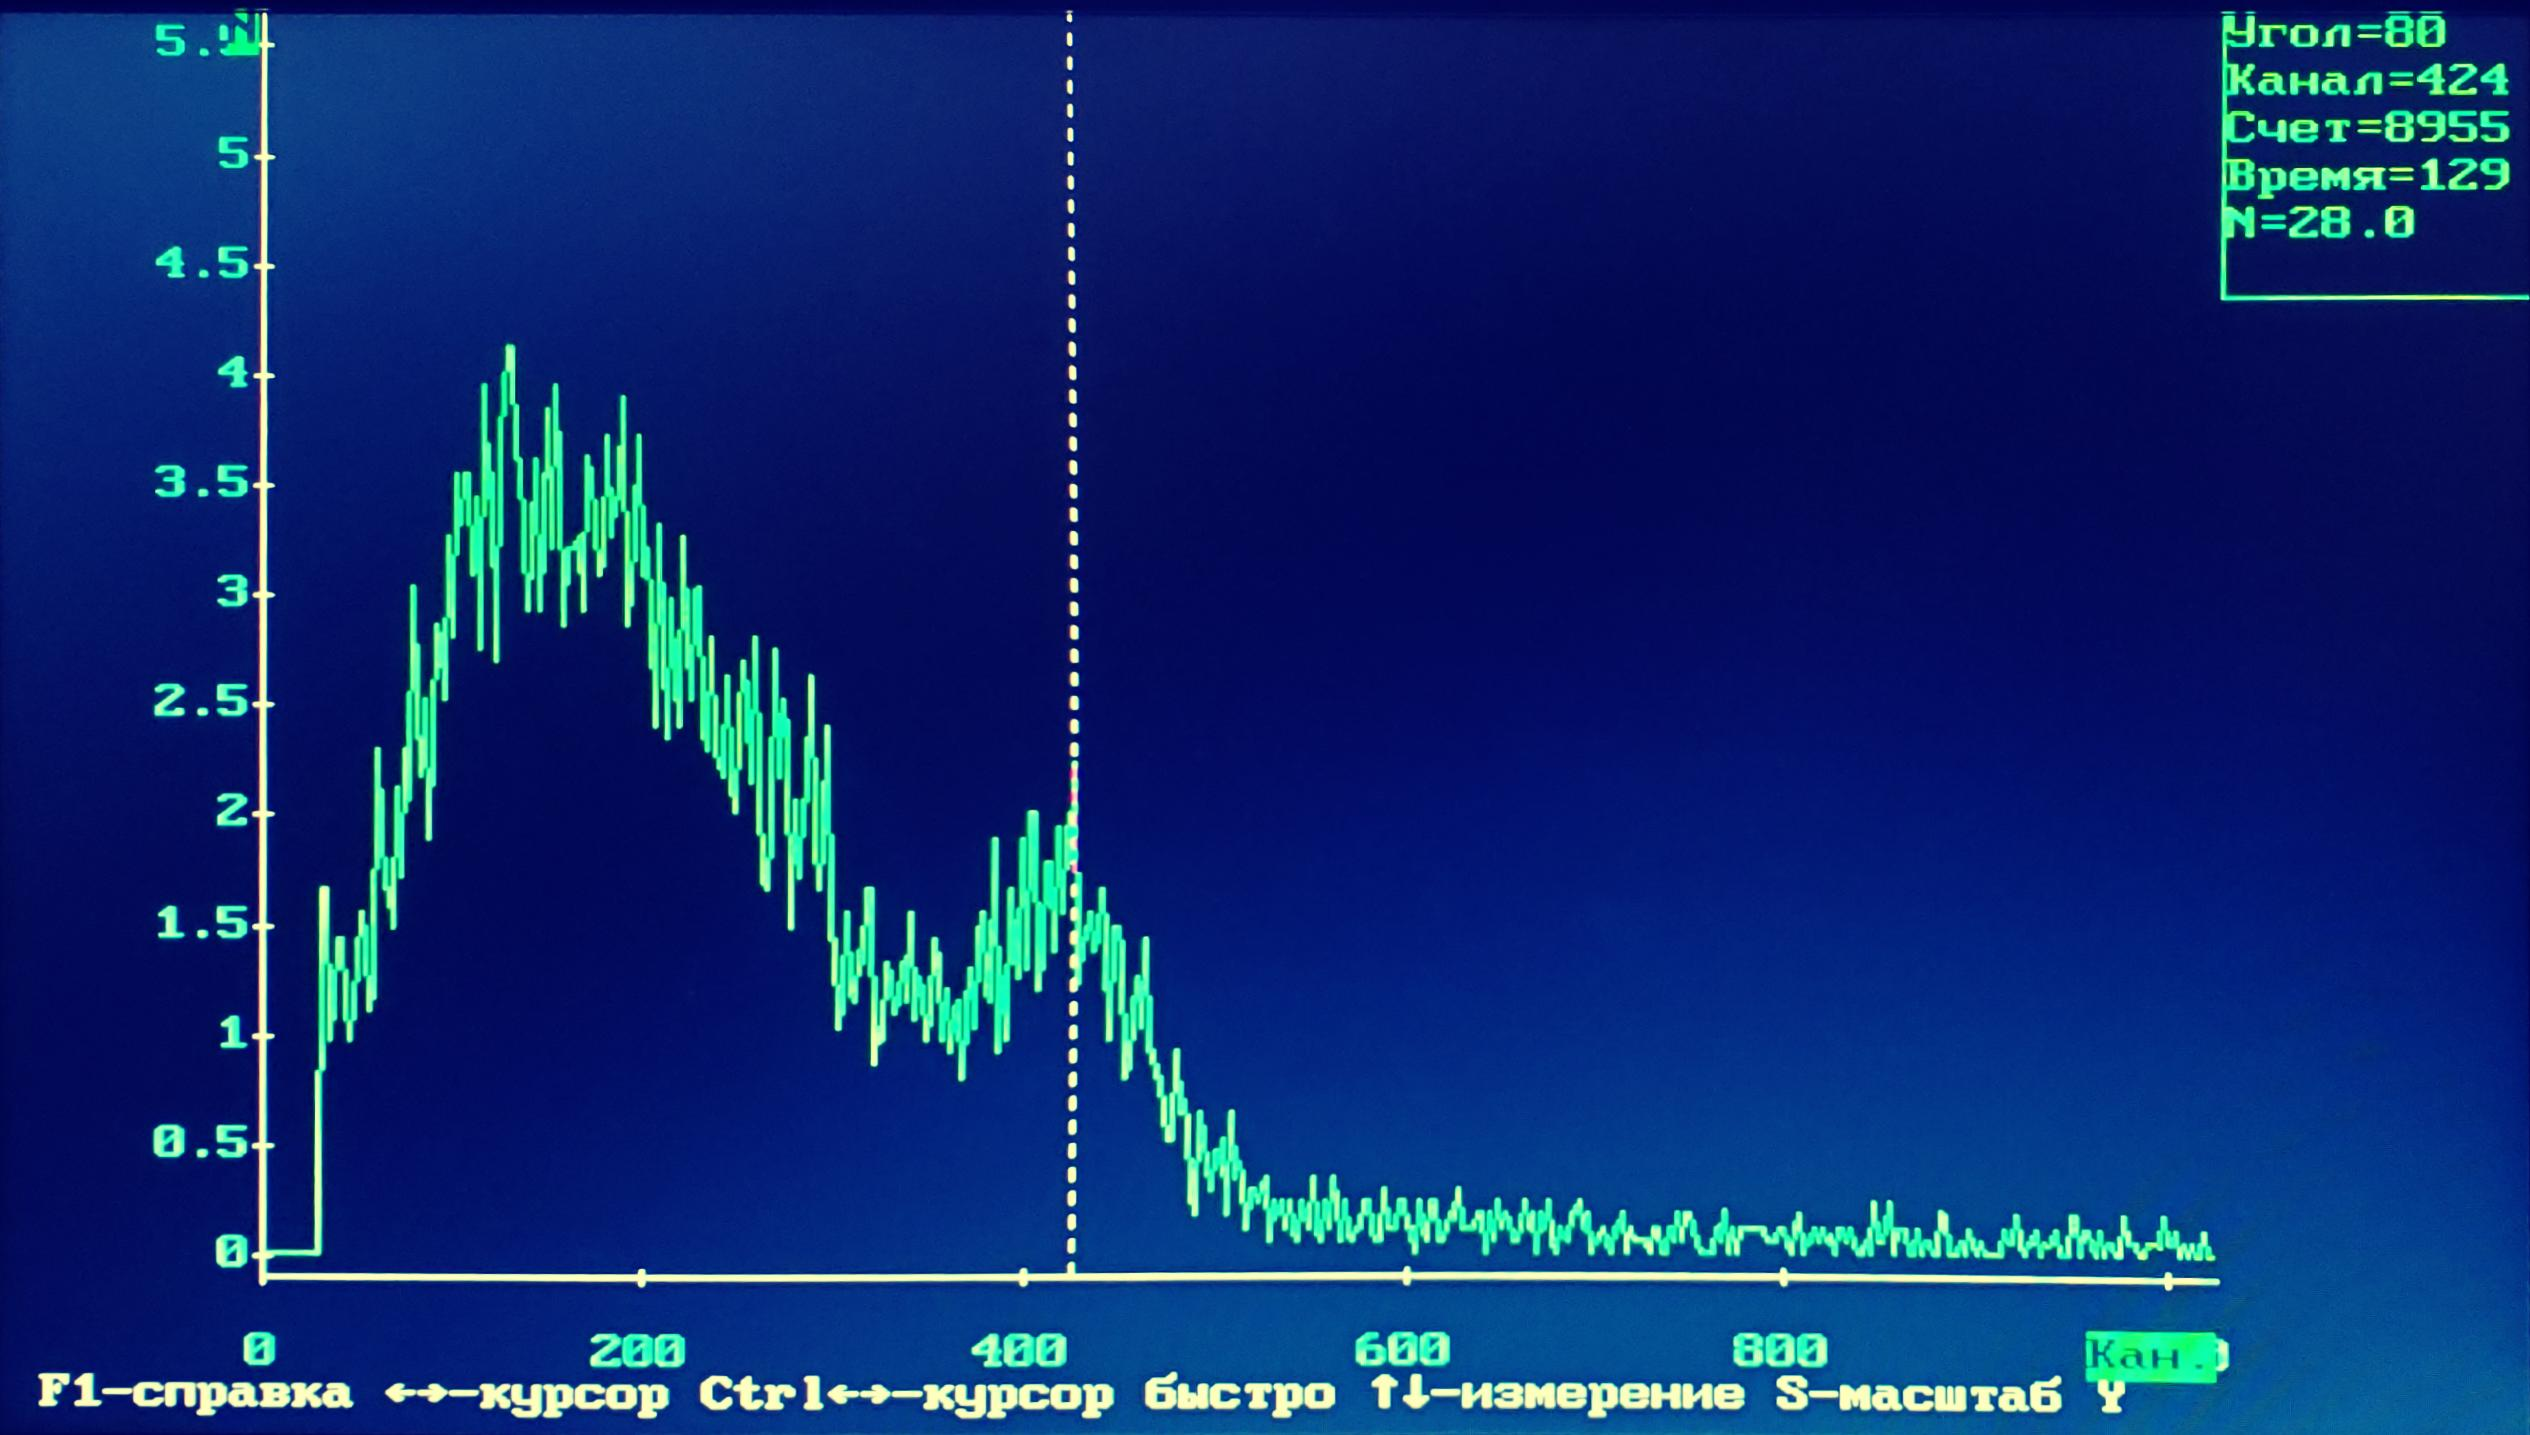
\includegraphics[width = \linewidth]{spectre80.jpg}}\\
      Рис 12. $\theta = 80^{\circ}$
    \end{minipage}
  \end{figure}
  \begin{figure}[h!]
    \begin{minipage}[h]{0.32\linewidth}
      \center{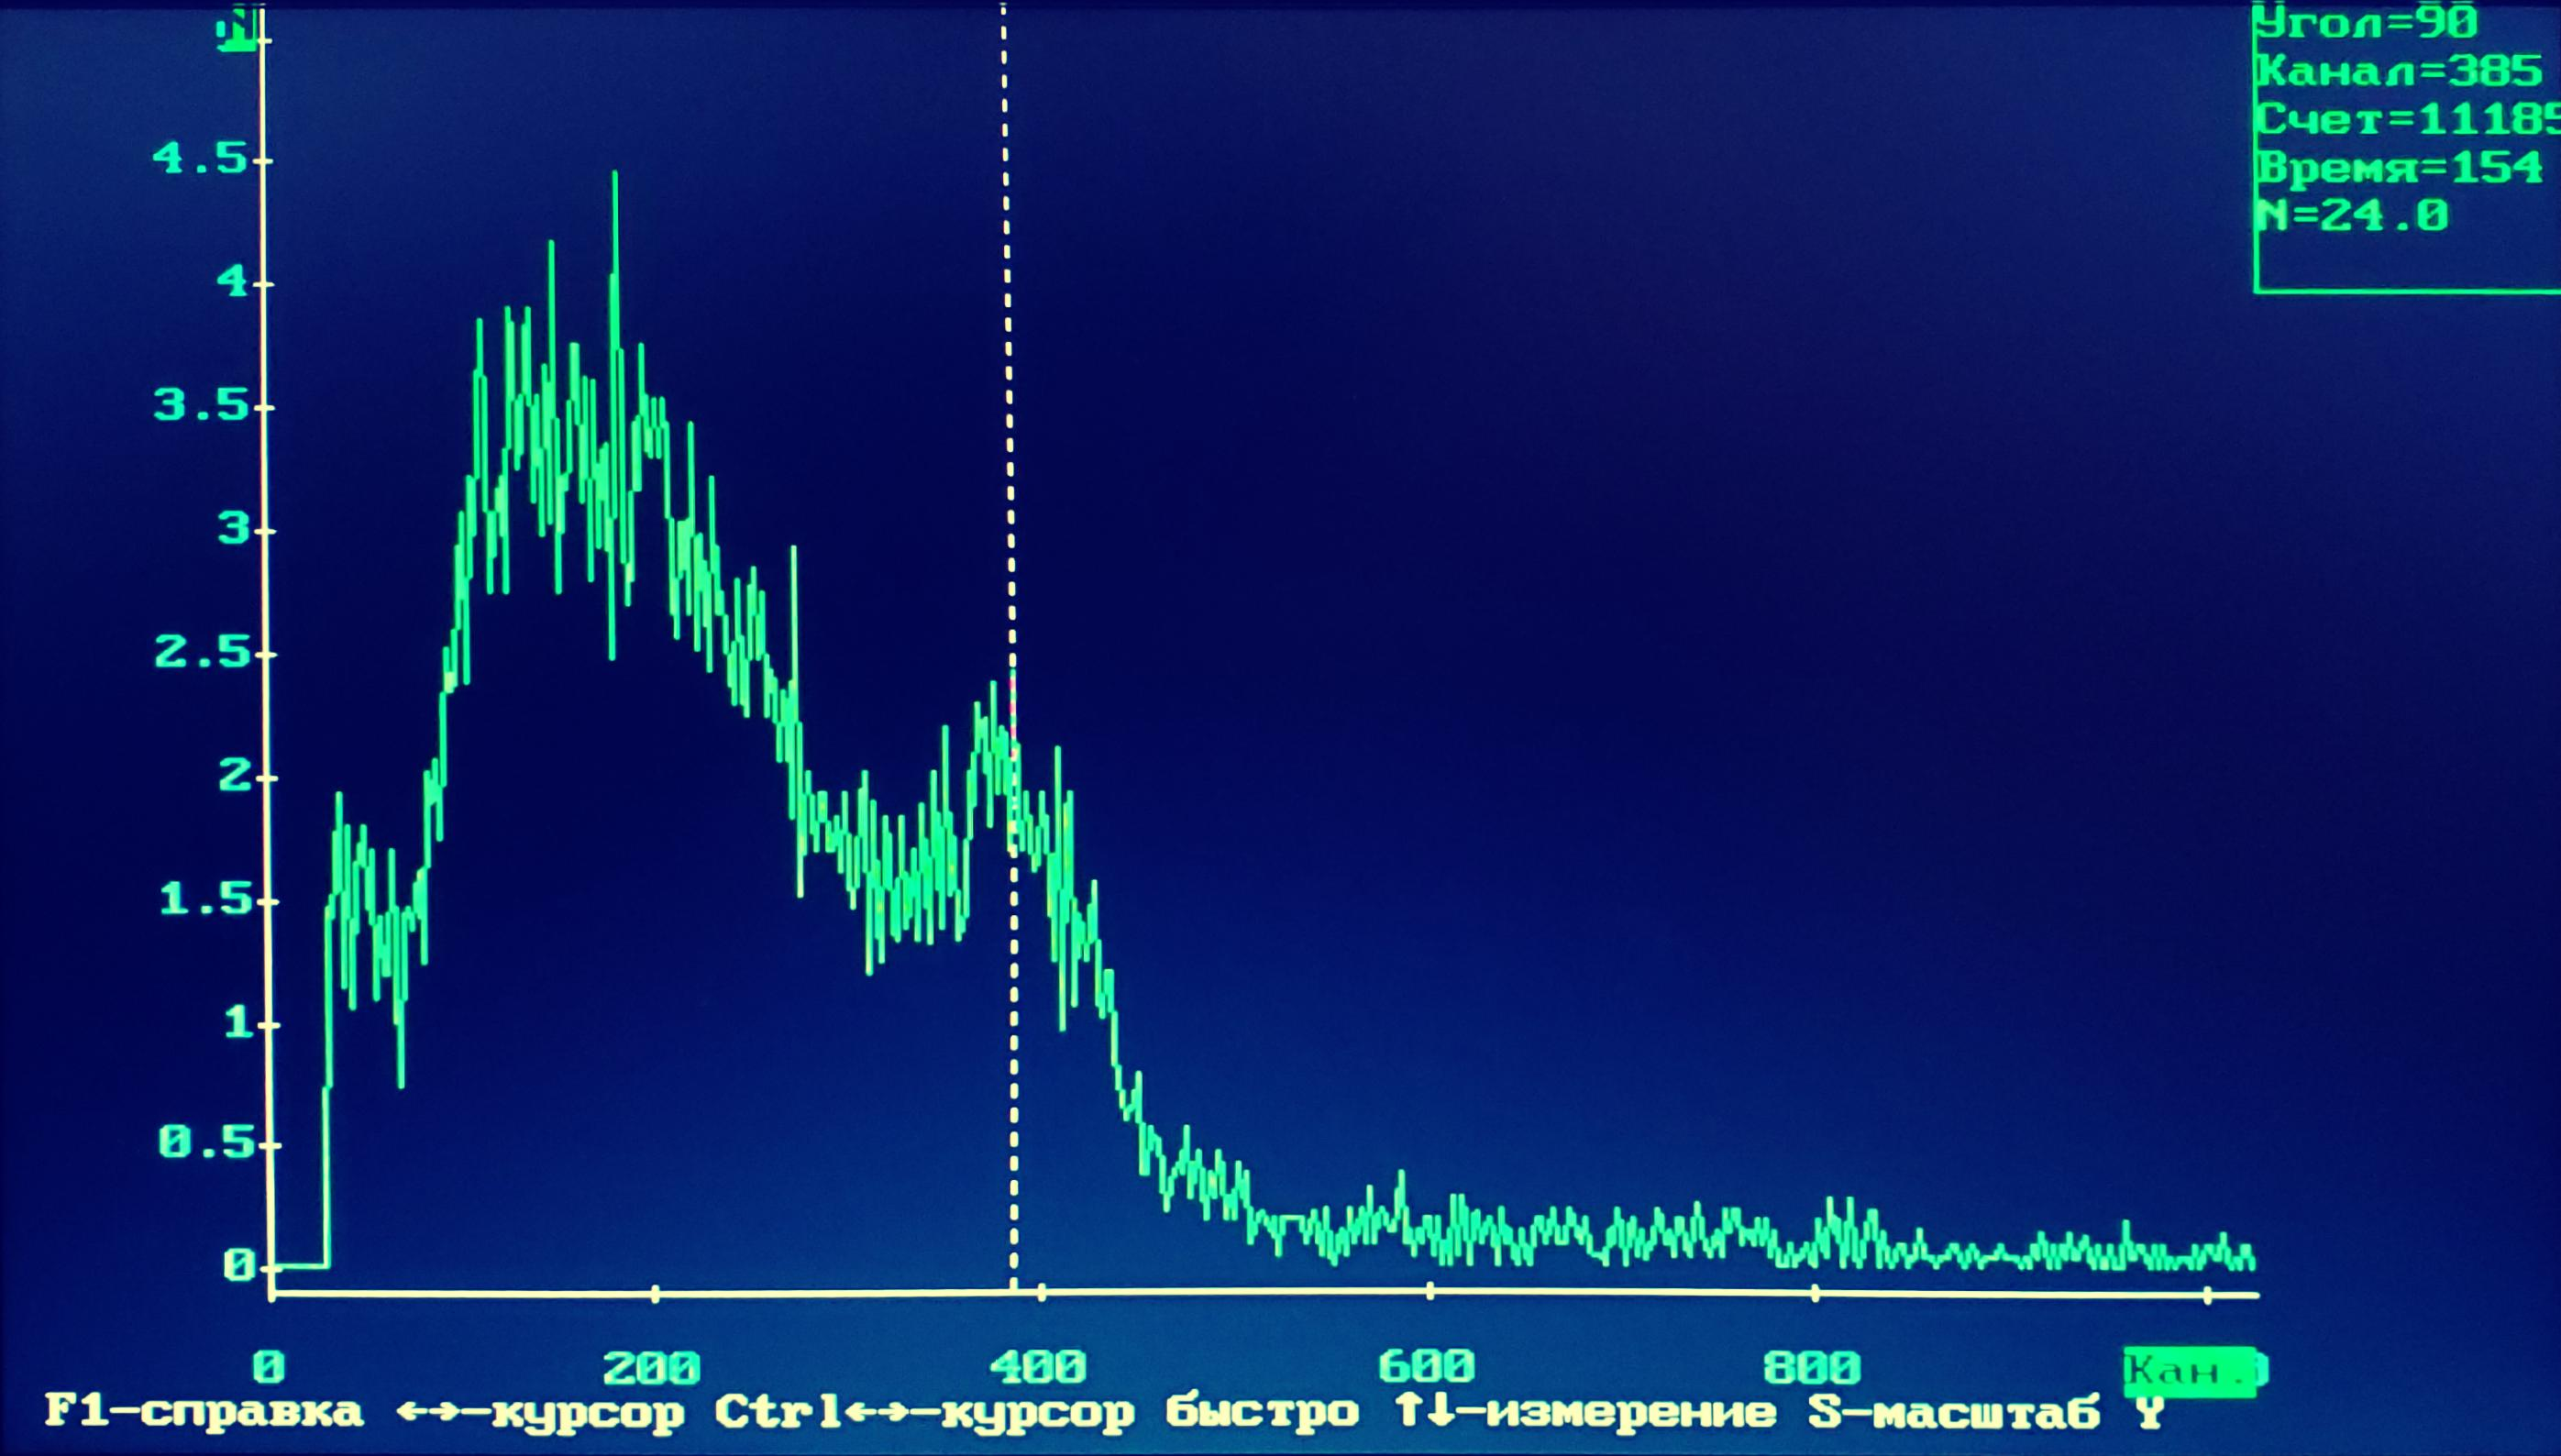
\includegraphics[width = \linewidth]{spectre90.jpg}}\\
      Рис 13. $\theta = 90^{\circ}$
    \end{minipage}
    \begin{minipage}[h]{0.32\linewidth}
      \center{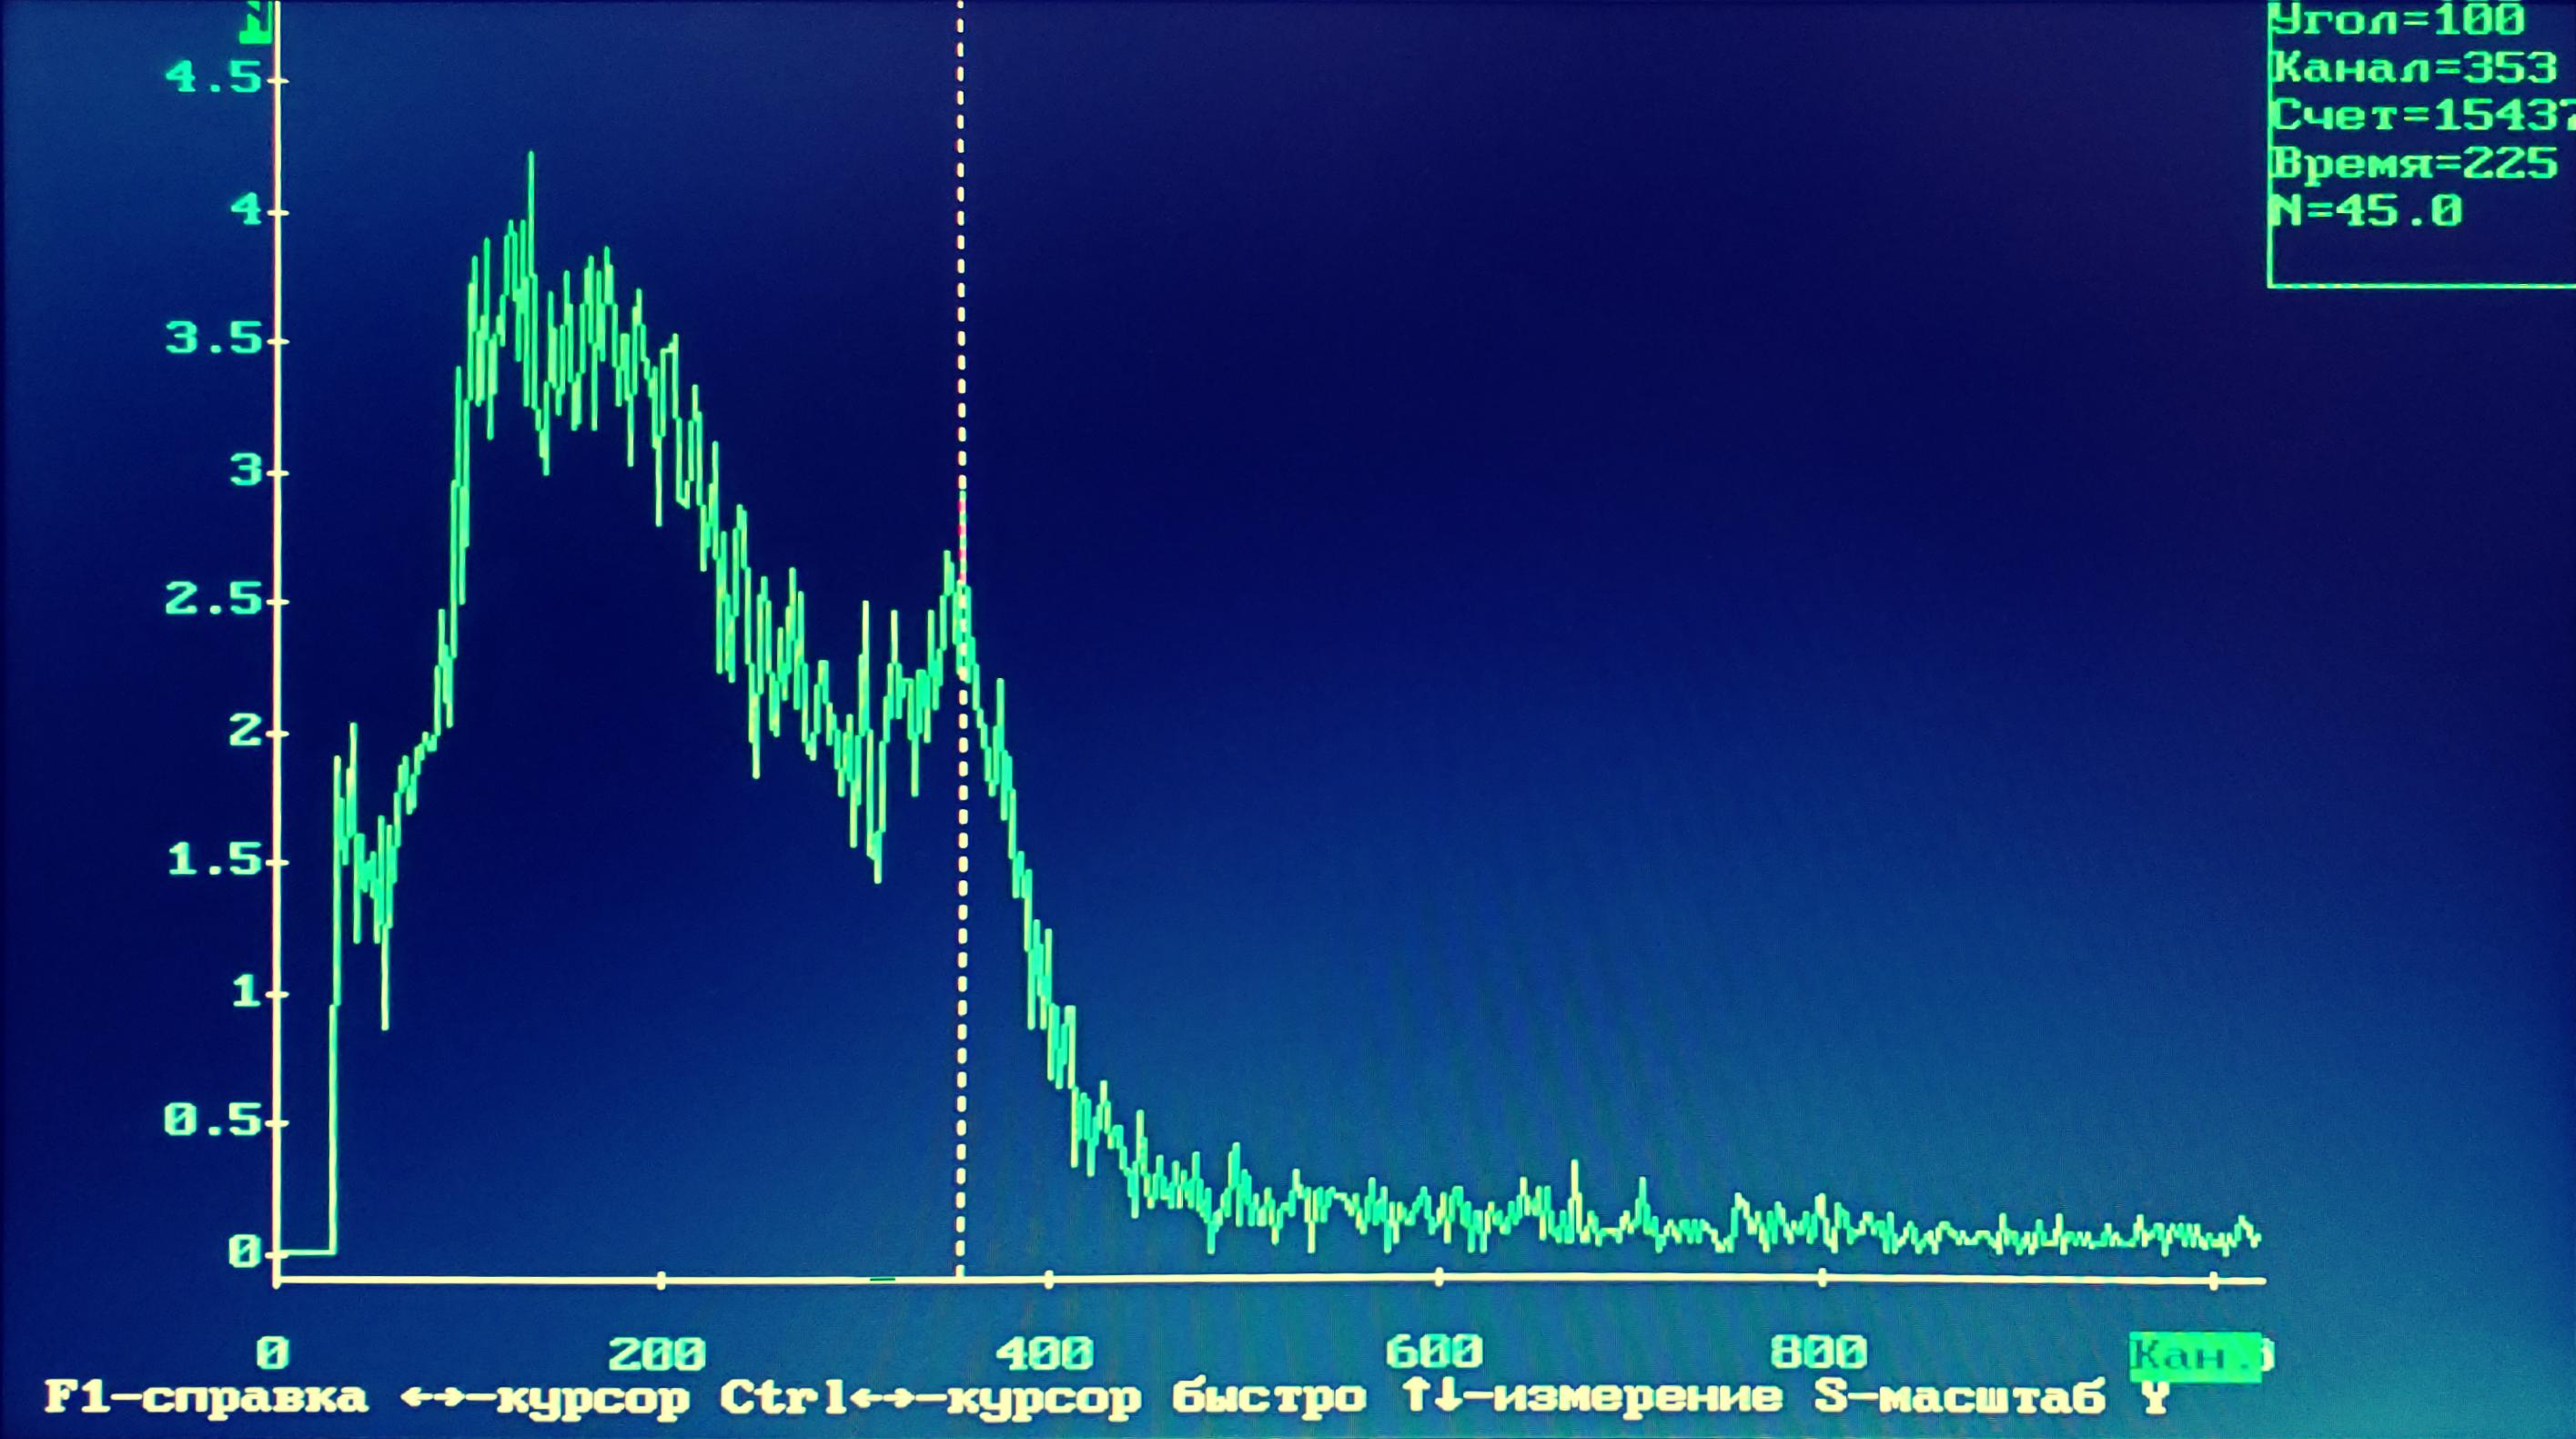
\includegraphics[width = \linewidth]{spectre100.jpg}}\\
      Рис 14. $\theta = 100^{\circ}$
    \end{minipage}
    \begin{minipage}[h]{0.32\linewidth}
      \center{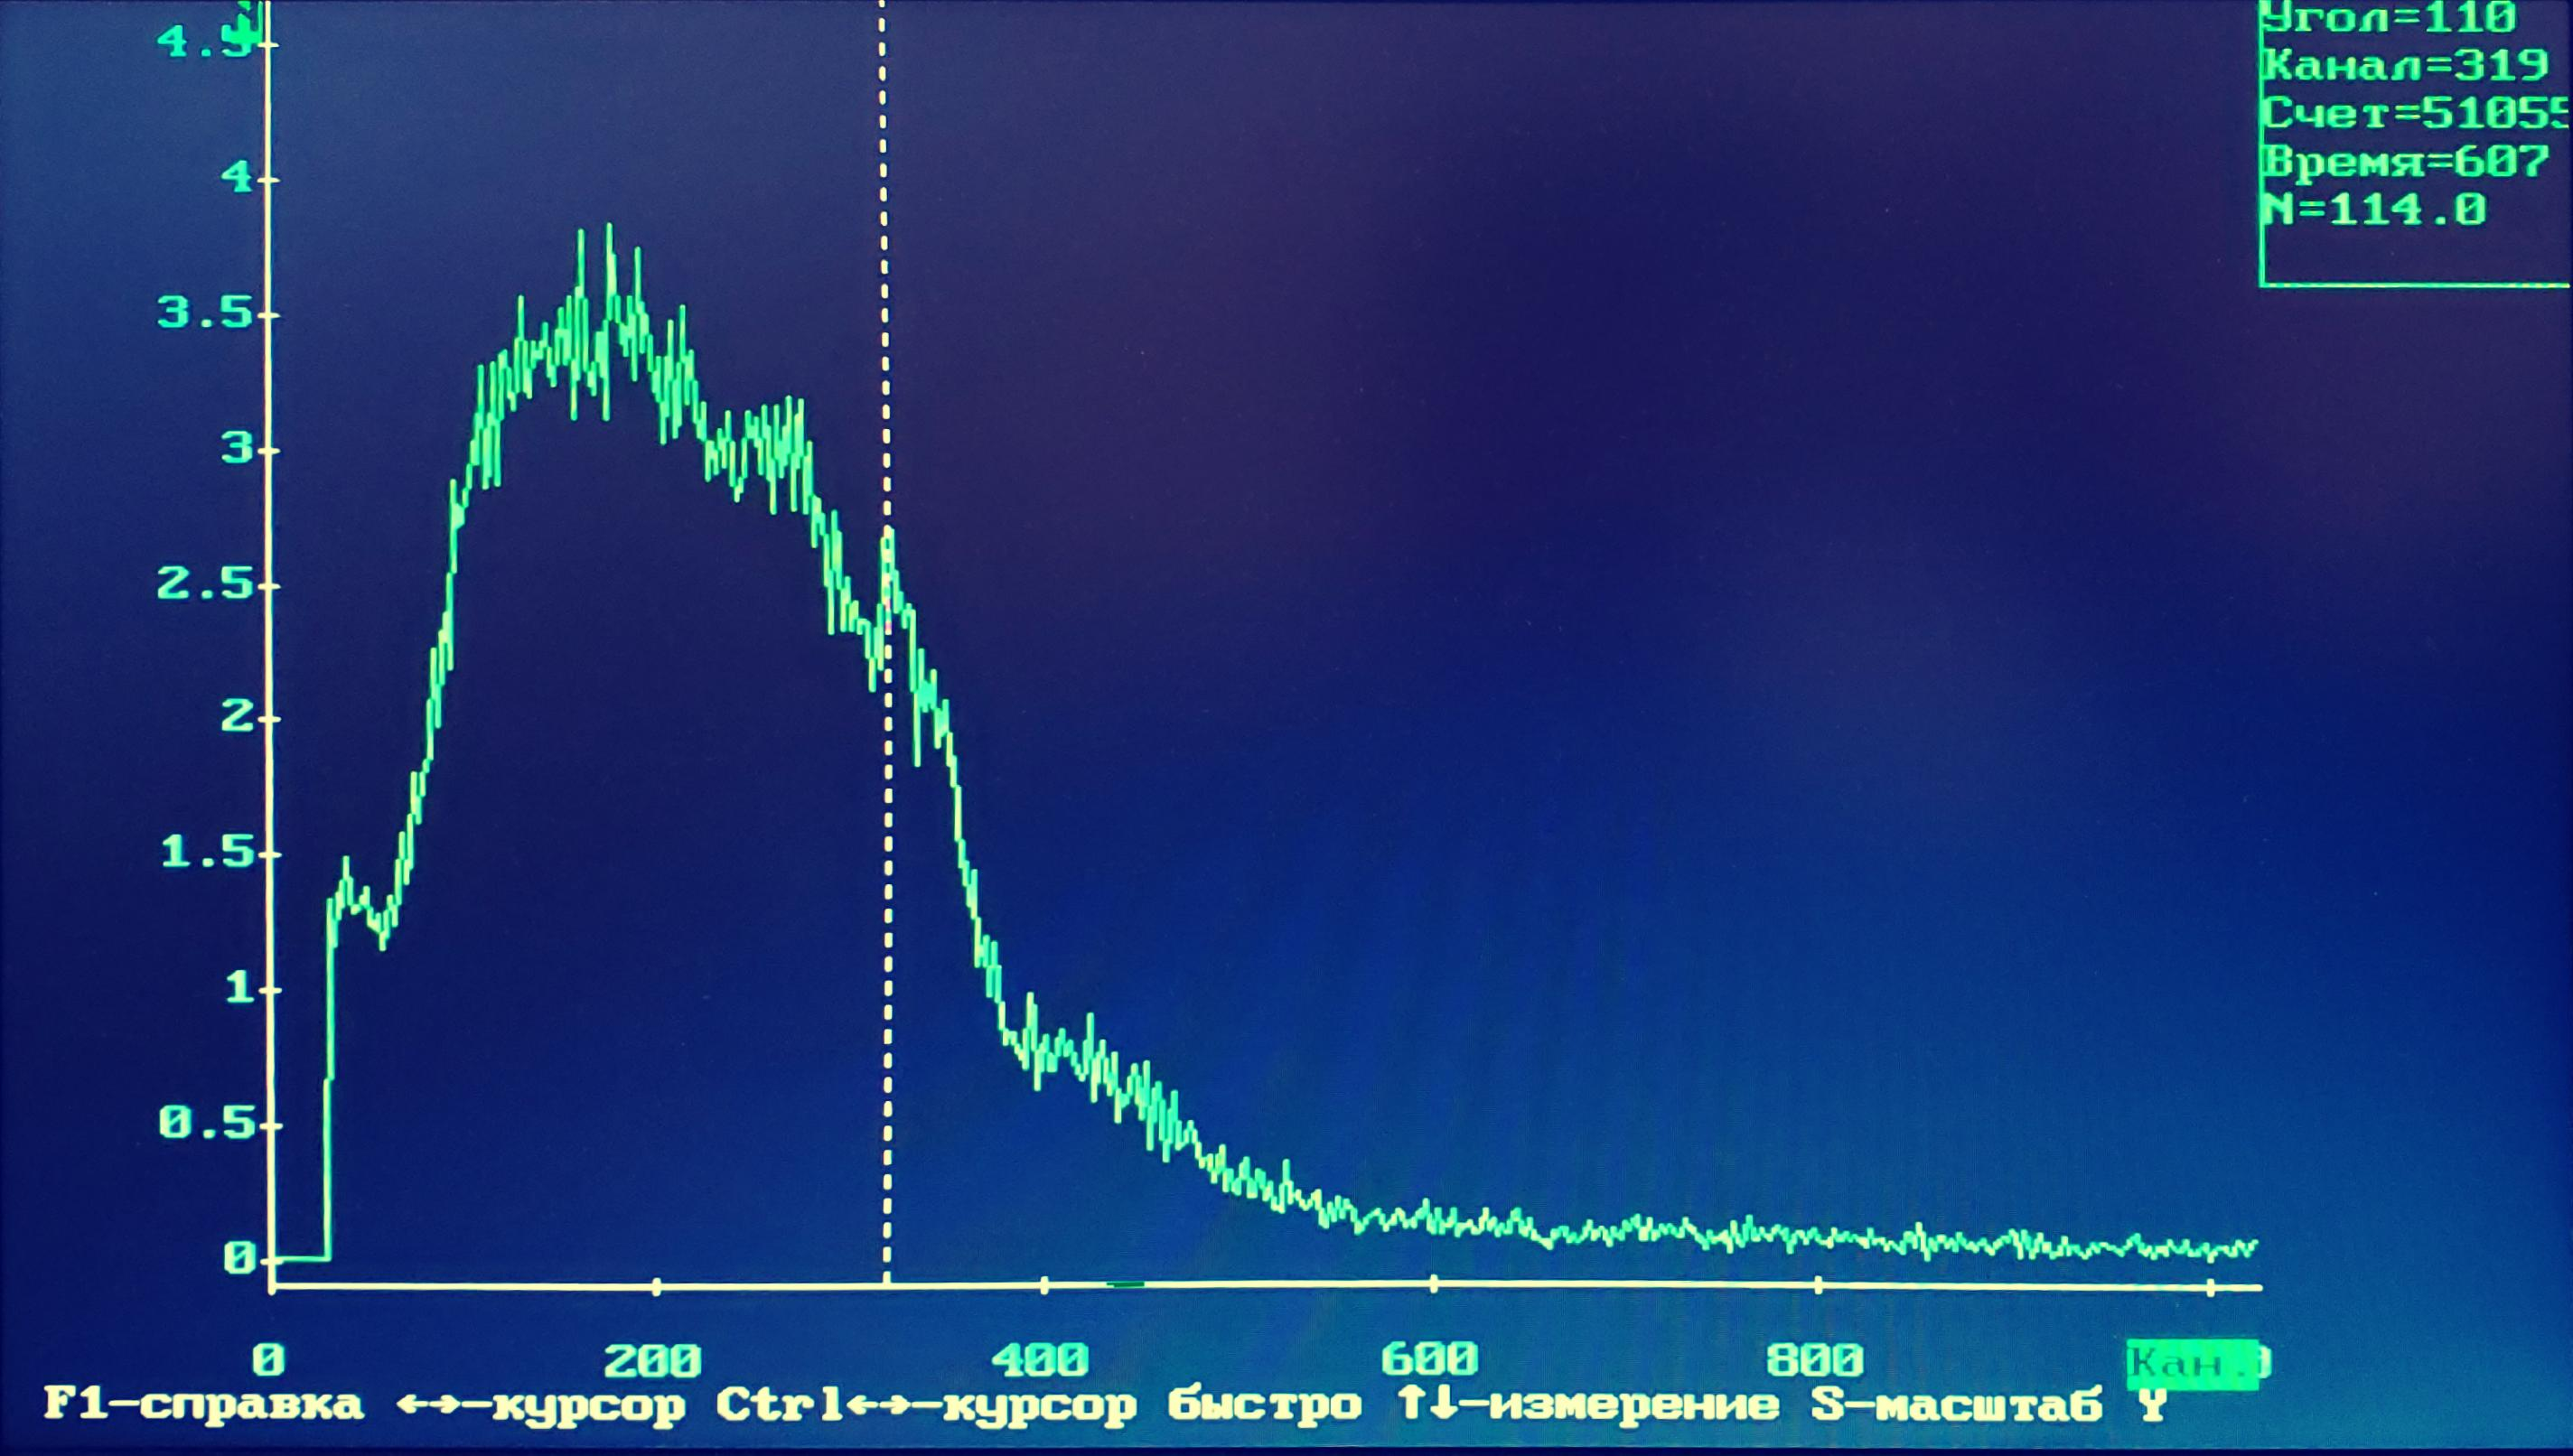
\includegraphics[width = \linewidth]{spectre110.jpg}}\\
      Рис 15. $\theta = 110^{\circ}$
    \end{minipage}
  \end{figure}
  \begin{figure}[h!]
    \begin{minipage}[h]{0.32\linewidth}
      \center{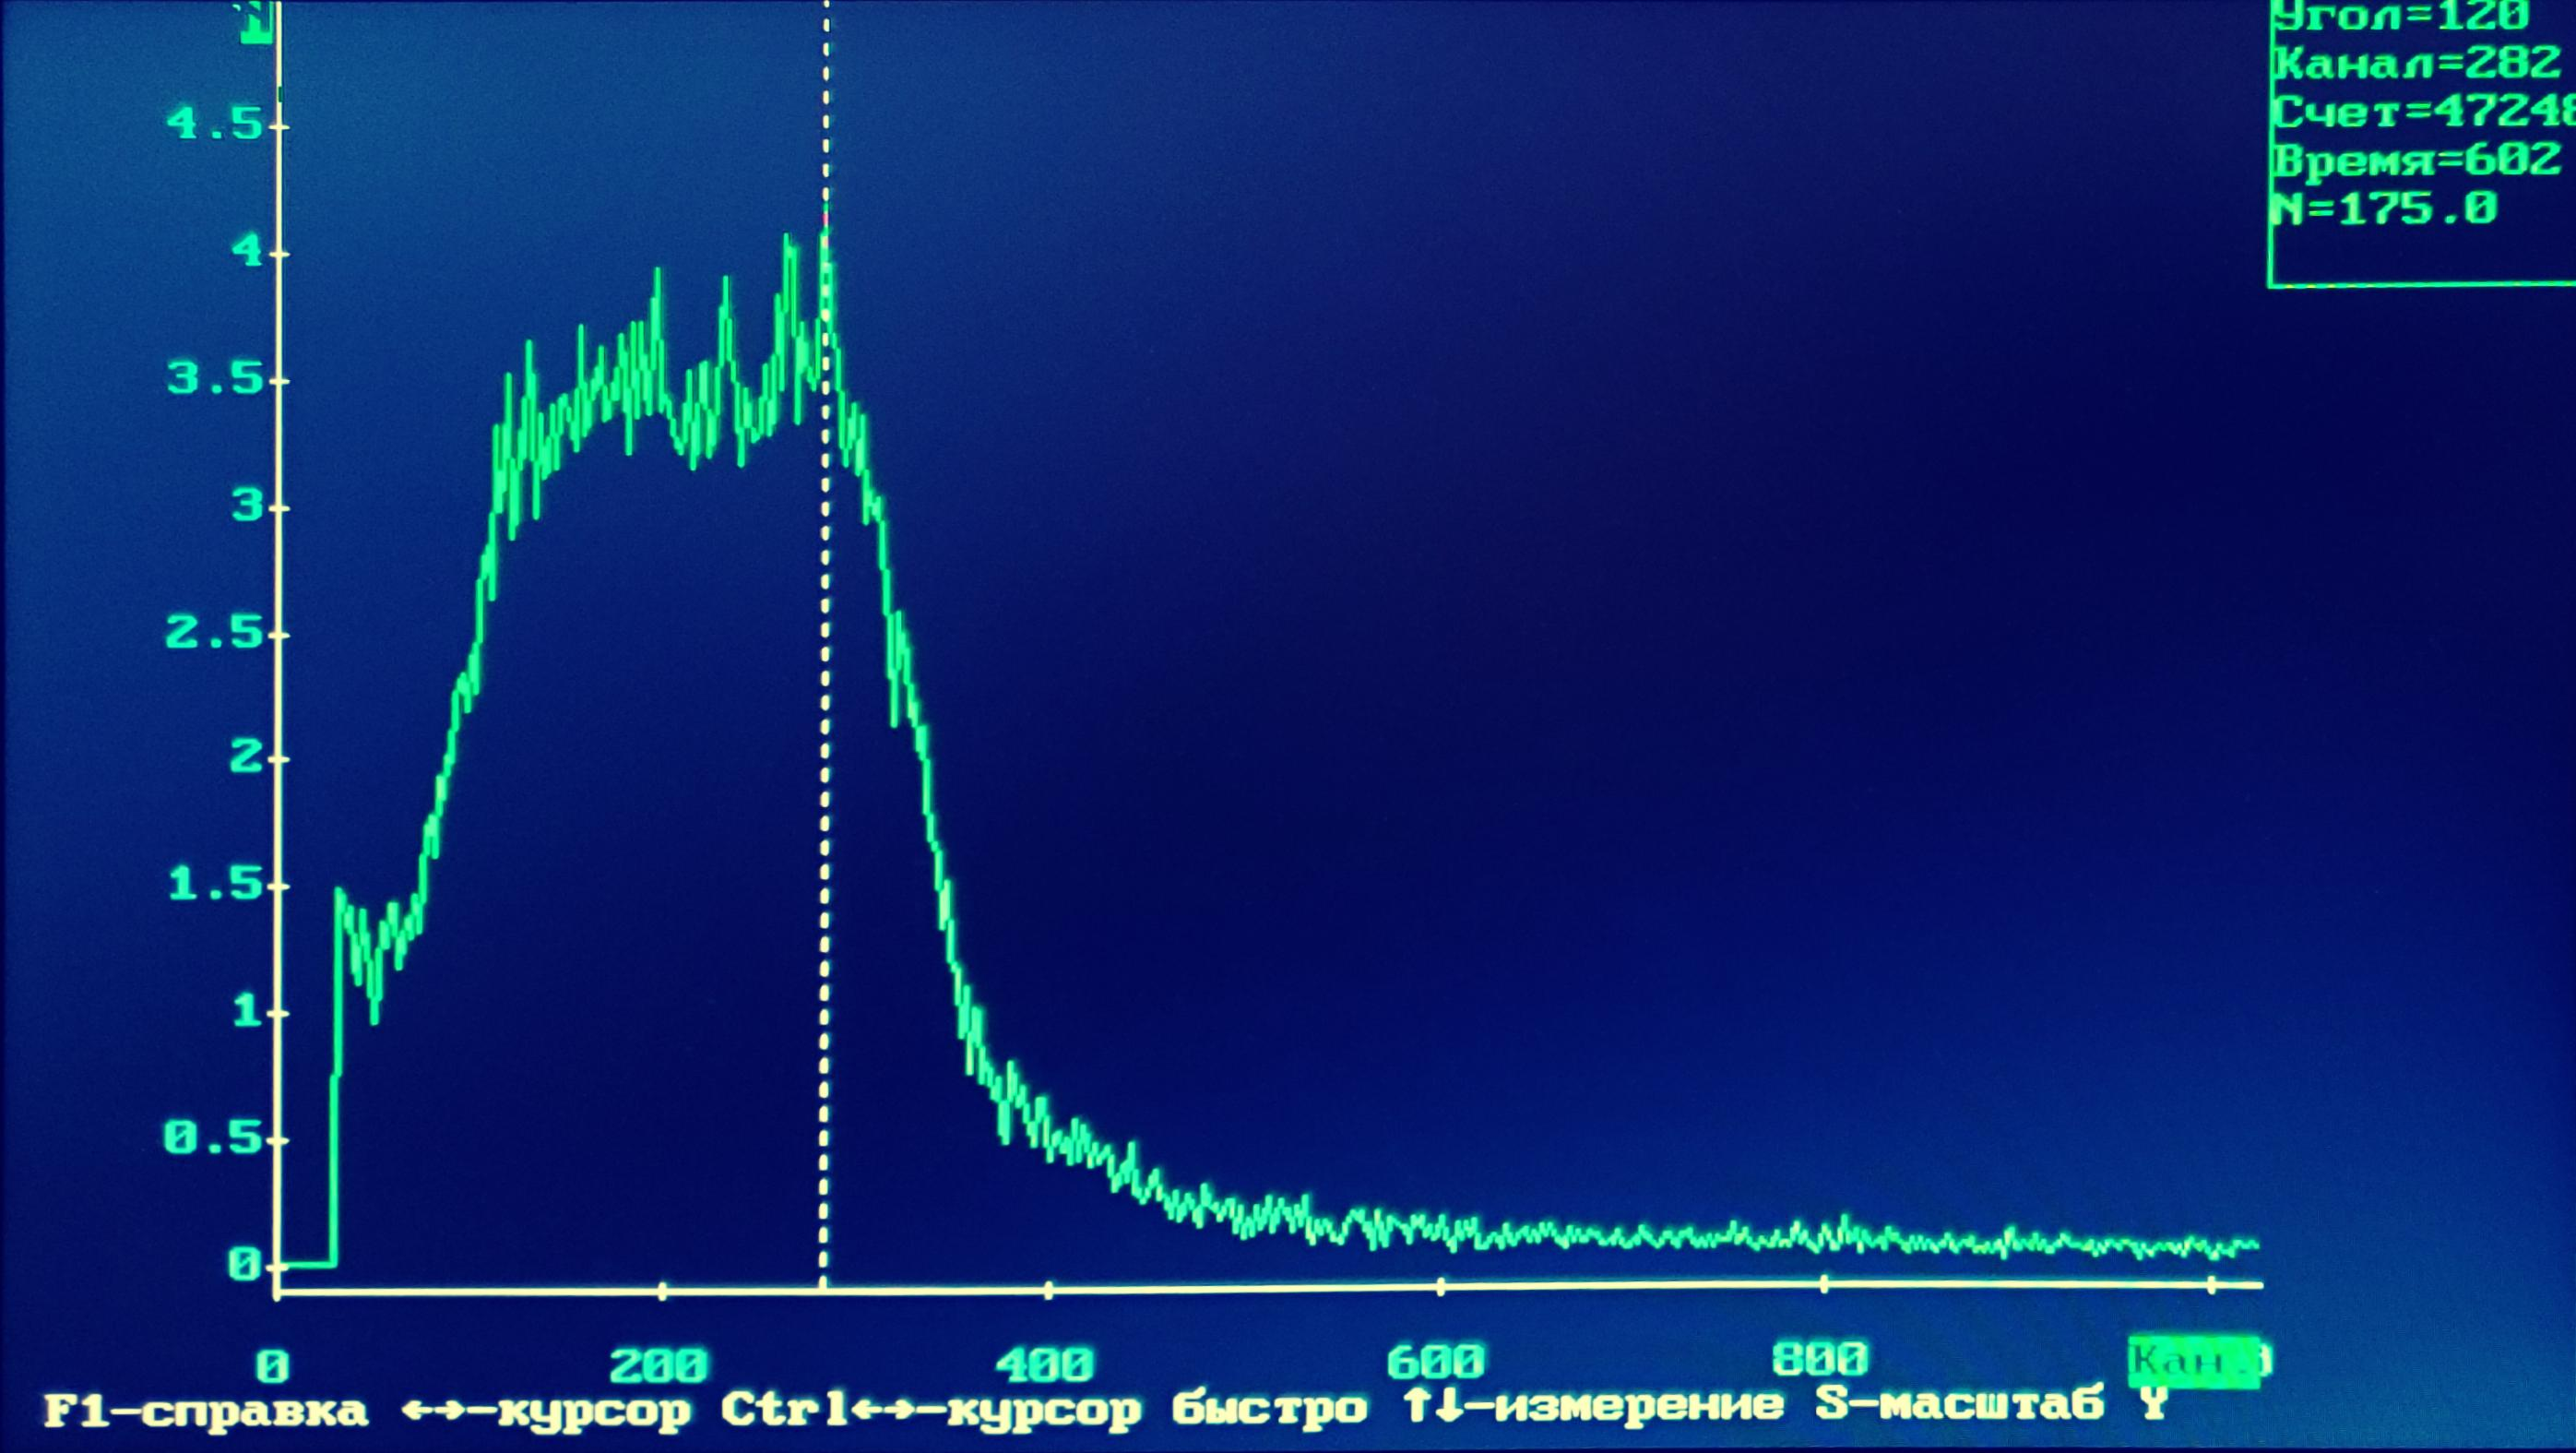
\includegraphics[width = \linewidth]{spectre120.jpg}}\\
      Рис 16. $\theta = 120^{\circ}$
      \label{fig:oscillograme}
    \end{minipage}
  \end{figure}

\end{document}
